% Need to discuss how we put data, the background estimate, and the signal model together
%     and make a claim as to the compatibility of the hypothesis with the data.
% Largely, this means I need to finally understand how pyhf actually works and what the hell the limit framework is doing.
\chapter{Results} \label{chapter:results}

%
%
%
%    I'm not sure I actually have to explain Baye's theorem here...
%    it doesn't appear to be obviously used, or if it is, we're implicitly using the "Uniform" Prior
%    Ask Steve
%
%    L gives probability of seeing the data we have, based on the given model.
%    We need the probability that the given model is the one responsible for the data we see.
%    i.e. we have P(data|model), but we need P(model|data)
%
%    To do this, we need Baye's rule, which comes from the basic 'anding' of probabilities:
%    P(a \& b) = P(a)*P(b|a) , or P(a \& b) = P(b)*P(a|b) . Thus
%    P(a)*P(b|a) = P(b)*P(a|b) 
%    P(b|a) = P(a|b) P(b) / P(a)
%    So we need P(model|data) = P(data|model) * P(model) / P(data)
%
%    For our data we have to use the extended L, which accounts for poisson stats.
%    Basic test is to test mu*S+B for what value of mu is compatible with data
%
%        
%
%
%Statistics is a powerful tool in science,
%    but one which can be very misleading if not used carefully.
%%The oft-used quote comparing lies and statistics exists for a reason;
%%    both can lead to incorrect scientific conclusions.
%%But whereas a lie can be caught by a simple slip of the tongue,
%%    it can take scientists years to discover a slight (intentional or not) mishandling of statistics.
%Unfortunately, the use of statistical methods is not optional.

%To begin, let me propose a much simpler experiment than the one described in this analysis.
%I have a coin, which I suspect may be biased to one side.
%How can I test this?
%A fair coin has a 50/50 chance of landing on either side.
%This means that, were I to flip the coin a large number of times,
%    I would expect a roughly equal number of heads and tails.
%Significant deviation from this ratio (e.g.\ 3 million heads to 1 million tails)
%    would indicate an obvious bias in the coin.
%The conclusion becomes far less obvious however, if the coin is flipped only a few times.
%Even if every flip comes up as heads, no meaningful conclusion can be made if the coin was only flipped e.g.\ four times.
%The crucial questions raised here, which statistical methods are able to address,
%    are how much data is needed to make a decisive statement about a hypothesis,
%    and what kind of statements can be made in lieu of that data.

%The first step to testing a hypothesis,
%    is to know precisely how \textit{likely} any particular outcome is based on that hypothesis.
%The hypothesis for the coin flip is that the probability $p$ of any given flip being heads is 50\%.
%For an experiment consisting of a number of flips $N$,
%    the overall probability of seeing an amount of heads $n$ is given by the binomial distribution:
%\begin{equation}
%    P(n|p) = \tinymatrix{N\\n} p^n (1-p)^{N-n}
%\end{equation}
%Where $P(n|p)$ is read as ``the probability of seeing $n$ heads \textit{given} their probability $p$.''
%With this, 
%
%basic binomial distribution (coin flip) allows obvious p-test. 
%Using a concrete toy example with numbers,
%Show a binomial PDF distro for N flips, and where on that distro the "data" lies
%Show a C-PDF, and again where the data is,
%    and explain that the "unlikeliness" can be used as a test metric, called a "p-value"
%Show of whether or not theory is compatible with data.


% NOTE: From here on, try to keep the p-value concept,
%   as well as the PDF and C-PDF, as a central focus.
% It's easy to conceptualize what a p-value is,
% so you should keep returning to it in order to retain 
% a concrete basis for all the weird math you're about to do
\section{Statistical Mathematics}

    I have thus far established how the analysis has collected its data,
        how it has estimated the amount of background present in those data,
        and how it has modeled the hypothesis for the HH process to be tested with those data.
    With these assembled, the final step is to arrange them together in order to make a definitive statement
        as to the validity or incompatibility of the hypothesis with the provided data.
    More plainly, the questions for this chapter are:
        was the di-Higgs process detected in the data,
        and what were the values of the $\kappa$ scale factors involved in its production?
    To answer these questions, I must turn to the field of statistical analysis.
    In this chapter, I want to explain why statistics is required for this analysis,
        discuss the specific statistical techniques this analysis uses,
        and conclude with what those techniques reveal in light of the data presented.

    % Introduce poisson statistics with single counting variable and only signal w/ toy example.
    % Discuss difference between coin toss and radioactivity.
    % i.e. that with a coin toss, the number to tosses is entirely determined by me, and is thus fixed.
    % For decay and such, the number of events is completely random, and what is fixed is how much time (luminosity)
    %     the experiment is given.
    Like most particle physics processes, the \vbfhhproc process results in a need to count outcomes,
        a fundamentally Poissonian situation.
    The number $n$ of di-Higgs process that are observed in ATLAS can then be modeled with a Poisson distribution\cite{cranmer2015practical}:
    \begin{equation}
        P(n|\nu) = \frac{ \nu^n e^{-\nu} }{n!}
        \,.
    \end{equation}
    This function $P(n|\nu)$ can be read as ``the probability $P$ of obtaining $n$ events \textit{given} the parameter $\nu$.''
    That is, for a process which is expected on average to produce $\nu$ number of events,
        this function gives the probability that such a process would produce $n$ events.

    The compatibility of a hypothesis with data can be established by use of a ``p-value test.''
    As an example, take the case of a simple alpha particle emitter with an unknown emission rate
        which I hypothesize emits radiation at a rate of once per minute.
    After one hour, I would expect on average 60 events.
    Running the experiment, I find that 52 events were detected.
    Plotting the Poisson distribution for $P(n|60)$ (Fig. \ref{fig:poisson_toy_sig:pdf}),
        I can see how likely an observation of 52 events is.
    \begin{figure}
        \centering
        \begin{subfigure}{0.48\textwidth} 
            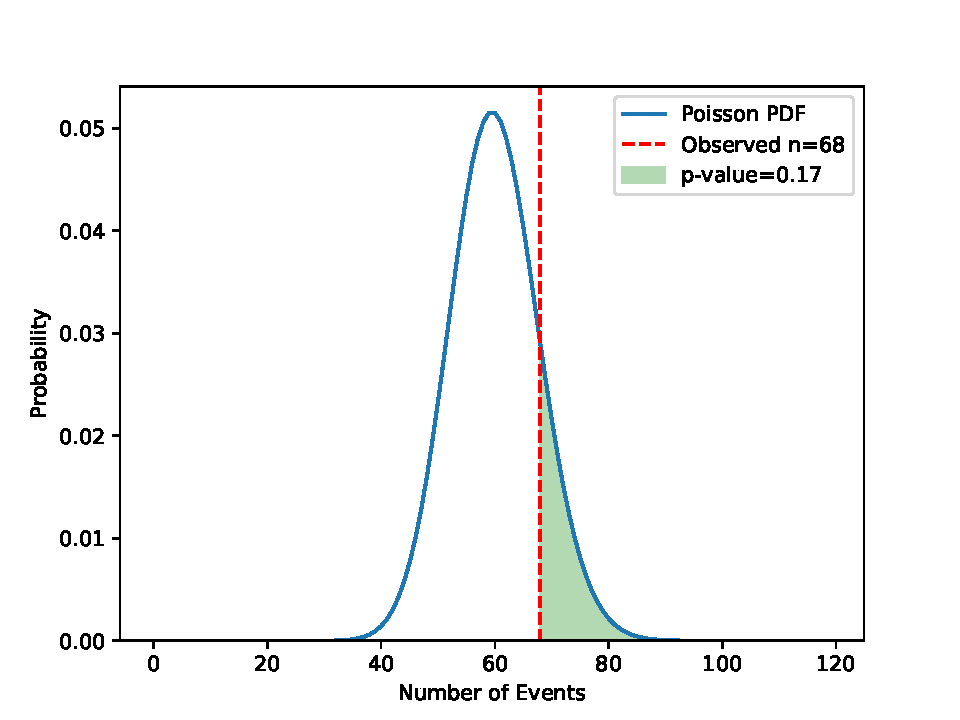
\includegraphics[width=\linewidth,height=\textheight,keepaspectratio]{results/toy_poisson}
            \caption{Toy Poisson PDF}
            \label{fig:poisson_toy_sig:pdf}
        \end{subfigure}
        \begin{subfigure}{0.48\textwidth}
            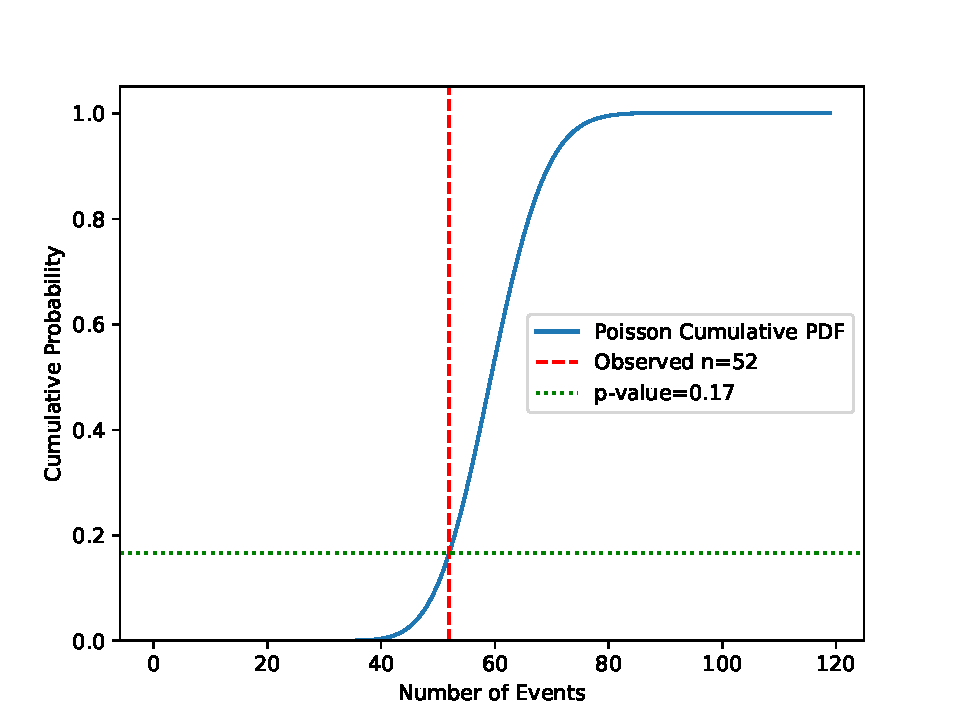
\includegraphics[width=\linewidth,height=\textheight,keepaspectratio]{results/toy_Cpoisson}
            \caption{Toy Poisson Cumulative PDF}
            \label{fig:poisson_toy_sig:Cpdf}
        \end{subfigure}
        \caption{
            A plot of the probability distribution function (PDF)
                and cumulative PDF for a toy Poisson experiment.
        }
    \end{figure}

    \FloatBarrier
    A ``p-test'' is the key tool that will be used throughout the rest of the analysis.
    Its goal is to find the probability that, were my hypothesis correct,
        I would obtain data with a value \textit{at least as extreme} as what I measured\footnote{
            There are actually several different variations of a p-test;
            this is specifically a one-sided p-test.
        }.
    So the p-value for an event rate of 52, given an expected average of 60, can be found by taking:
    \begin{equation}
        \textrm{p-value}(N=52) = P(0|60) + P(1|60) + ... + P(51|60) ... P(52|60) = \sum\limits_{n=0}^N P(n|60)
        \,.
    \end{equation}
    This is best visualized using the \textit{cumulative} probability distribution function (Fig. \ref{fig:poisson_toy_sig:Cpdf}).
    In this example, the p-value would be 0.17.
    A typical standard for many statistical tests, and the one used in this analysis,
        is to establish a ``Confidence Level'' (CL) in the results of an experiment at a level of 95\%. 
    The confidence level is simply $1-p$, so a CL of 0.95 corresponds to a p-value of less than 0.05.
    Because this toy experiment has a p-value larger than 0.05,
        the conclusion would be that ``the hypothesis was compatible with the data within a CL of 95\%.''


    % Introduce background
    % Ditch toy, pull out actual Background and Signal (SM) event yields.
    % Should also probably dig up the "sensitivity" metric and show how bad that is here as well.
    % CLs = CLs+b/CLb explained in (Barlow:2019svl pg. 192)
    % The abysmal performance here should justify splitting the event into bins,
    %     in order to identify regions of Mhh that we are more sensitive to.
    % Using multiple bins however, dramatically complicates the statistical analysis.
    % Enter the profile likelihood fit.
    Moving on from the toy example, the hypothesis being tested in this analysis
        involves a background event rate in addition to the signal hypothesis being considered.
    The average number of events expected is then $\nu = S + B$,
        where $S$ and $B$ are the signal and background rate yields respectively.
    The confidence limits in such a situation are handled in different ways from one analysis to another,
        but in this analysis the p-value of the signal alone is given by
    \begin{equation}
        P_S = \frac{P_{S+B}}{1 - P_B}
        \,.
    \end{equation}
    Where $P_{S+B}$ is the p-value of the hypothesis assuming the signal is present,
        and $P_B$ is the p-value of the background-only hypothesis
        (often called the ``null hypothesis,'' $H_0$)\cite{Barlow:2019svl}.
    $P_S$ then provides a probability which is relative to the ability of the null hypothesis to explain the observed effects by itself.
    For example, in the case where the observed number of events is far larger than the background estimate,
        such that the background is entirely unable to account for the observation,
        $P_B$ will be approximately 1, and $1-P_B$ will approach 0.
    This will in turn scale $P_{S+B}$ up dramatically,
        emphasizing that since the background is unable to describe the observation
        the signal is more likely to be present to account for the difference.

    \begin{table}[tbh]
       \begin{center}
           \caption{Estimated and Observed Event Yields}
           \label{tab:event_yield}
           \footnotesize
           \begin{tabular}{|l|l|}
           \toprule
               Type  &	Event Yield \\
               \midrule
               Signal Hypothesis (SM) & 0.36 \\
               Signal Hypothesis (\kvv=3) & 52.7 \\
               Background Estimate  & 493.6 \\
               Observed Data & 495 \\
           \bottomrule
           \end{tabular}
       \end{center}
    \end{table}

    The total yields of the data, background estimate, and the SM and \kvv=3 signal hypotheses are provided in Table \ref{tab:event_yield},
        and their PDF and cumulative PDFs can be seen in Fig. \ref{fig:poisson_sig_kvv1_pdf} and \ref{fig:poisson_sig_kvv1_Cpdf}.
    Proof of the di-Higgs process would necessitate an excess of events so significant that
        the null hypothesis must be rejected (typically $P_B < 10^{-7}$, the ``$5\sigma$'' discovery limit).
    Here though, the background estimate almost completely overlaps with the observed data,
        resulting in a $P_B = 0.55$.
    This means the null hypothesis is highly compatible with the data and cannot be rejected.
    Since the null hypothesis cannot be rejected (and thus the di-Higgs process cannot be directly measured)
        the next best thing that can be done is to instead reject variations of the signal hypothesis.
    Setting \kvv to three times the SM value has a drastic effect on the hypothesized signal yield,
        which would have been significant in the observed data were this the true value.
    The complete lack of any noticeable deviation from the background-only hypothesis (Fig. \ref{fig:poisson_sig_kvv3_pdf})
        thus results in the low signal p-value of 0.03 (Fig. \ref{fig:poisson_sig_kvv3_Cpdf}).
    As this falls below the 0.05 cutoff, I can state with 95\% confidence that \kvv=3 (with \kl and \kv equal to 1)
        can be excluded from the realm of realistic scenarios.
    On the other hand, the SM signal has a p-value which exceeds 1.
    This is mostly a quirk of how the signal p-value is defined,
        but indicates that the signal hypothesis is highly compatible with the observed data,
        in this case because the signal is so tiny as to practically be a rounding error.

    \begin{figure}
        \centering
        \begin{subfigure}{0.48\textwidth} 
            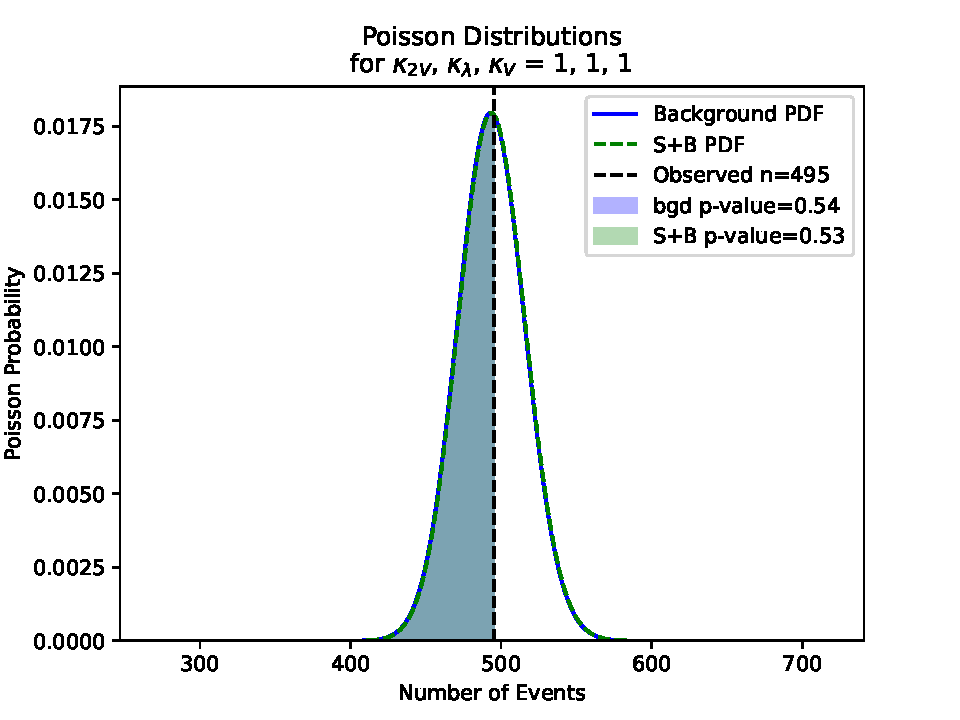
\includegraphics[width=\linewidth,height=\textheight,keepaspectratio]{results/total_yield_poisson_1p00_1p00_1p00}
            \caption{}%Poisson PDF for \kvv = 1}
            \label{fig:poisson_sig_kvv1_pdf}
        \end{subfigure}
        \begin{subfigure}{0.48\textwidth}
            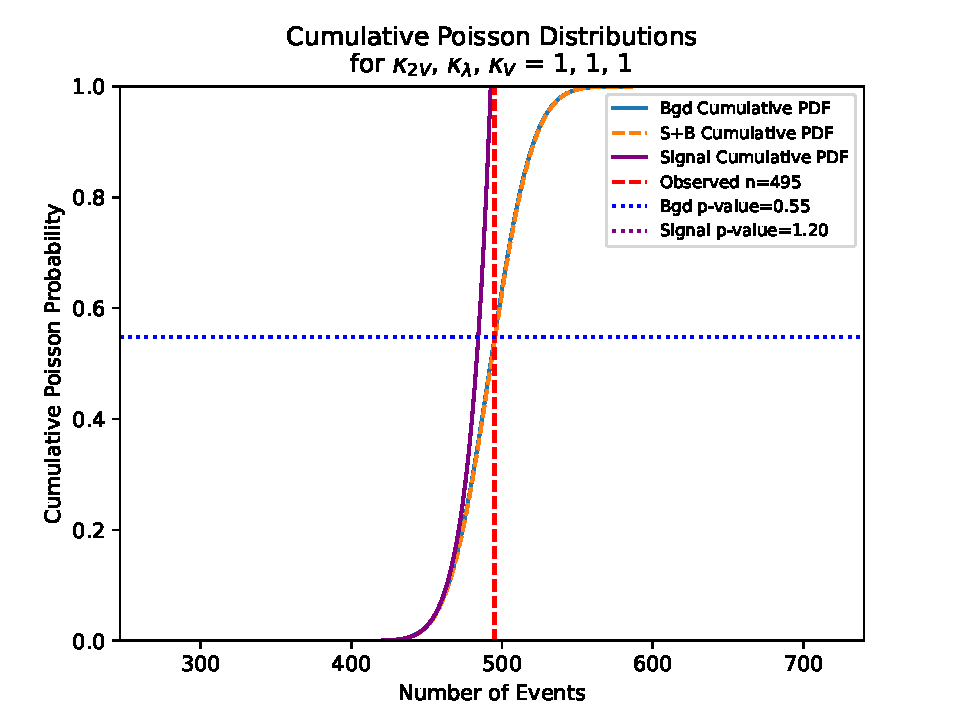
\includegraphics[width=\linewidth,height=\textheight,keepaspectratio]{results/total_yield_Cpoisson_1p00_1p00_1p00}
            \caption{}%Poisson Cumulative PDF for \kvv = 1}
            \label{fig:poisson_sig_kvv1_Cpdf}
        \end{subfigure}\\
        \begin{subfigure}{0.48\textwidth} 
            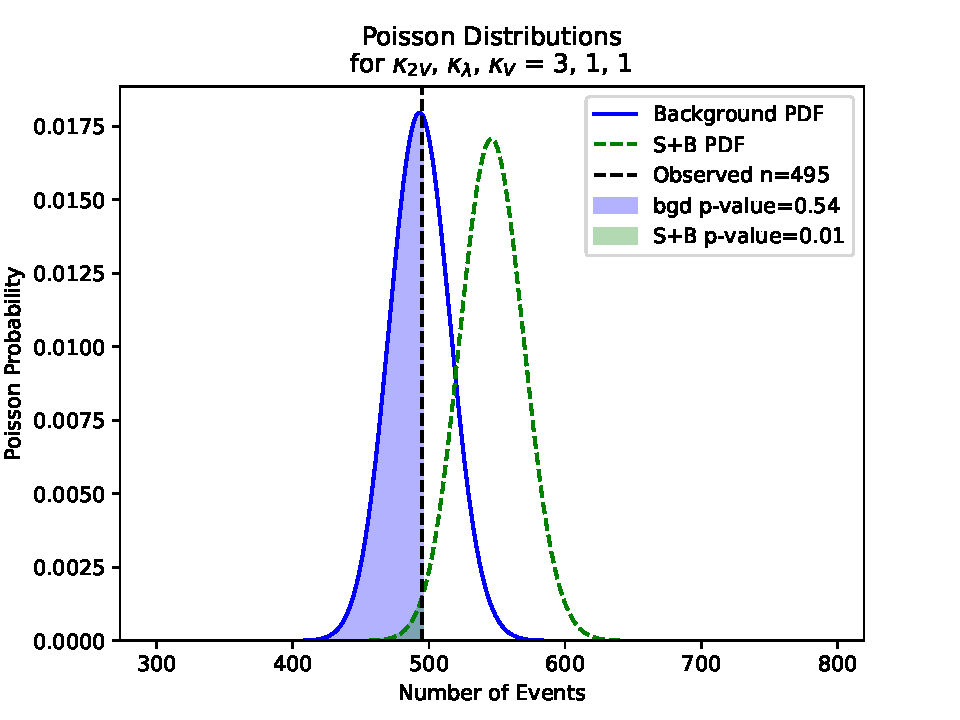
\includegraphics[width=\linewidth,height=\textheight,keepaspectratio]{results/total_yield_poisson_3p00_1p00_1p00}
            \caption{}%Poisson PDF for \kvv = 3}
            \label{fig:poisson_sig_kvv3_pdf}
        \end{subfigure}
        \begin{subfigure}{0.48\textwidth}
            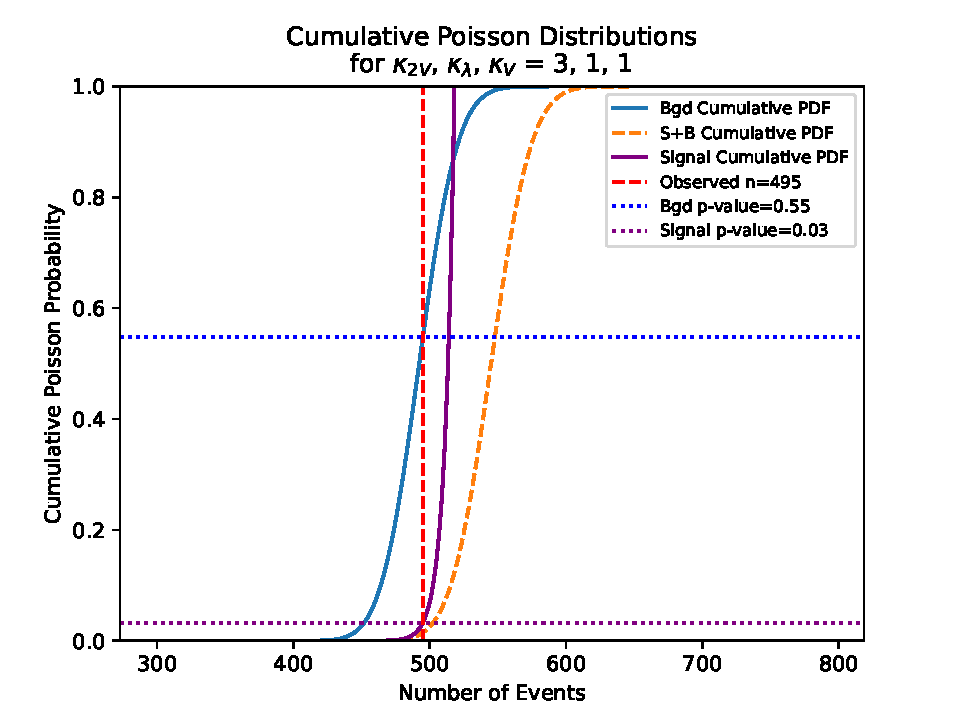
\includegraphics[width=\linewidth,height=\textheight,keepaspectratio]{results/total_yield_Cpoisson_3p00_1p00_1p00}
            \caption{}%Poisson Cumulative PDF for \kvv = 3}
            \label{fig:poisson_sig_kvv3_Cpdf}
        \end{subfigure}
        \caption{
            A plot of the probability distribution function (PDF)
                and cumulative PDF for the estimated background and simulated signal,
                with the observed yield denoted in both.
        }
    \end{figure}

    A useful technique for visualizing the compatibility of a signal hypothesis with data is to use a ``$\mu$ scan.''
    With this technique the expectation value is subtly adjusted to be $\nu = \mu S + B$,
        where $\mu$ now acts a scaling factor to the signal yield.
    The p-tests shown above can then be repeated for a variety of values of $\mu$,
        with the critical $\mu$ value identified as that which produces a signal p-value of 0.05.
    Figures \ref{fig:muscan_kvv1} and \ref{fig:muscan_kvv3} show such a test for \kvv set to 1 and 3.
    In a sense, what these figures state is how much the proposed signal would have to be scaled in order to be realistically perceivable.
    For \kvv = 1, this means that the signal would need to be scaled by a factor of 134 before it would make a noteworthy impact against the background.
    In contrast, the plot for \kvv = 3 highlighting a $\mu$ of 0.91 indicates
        that the signal would have to be \textit{reduced} to 91\% of its yield before it could be considered as reasonably compatible with data.

    \begin{figure}
        \centering
        \begin{subfigure}{0.48\textwidth} 
            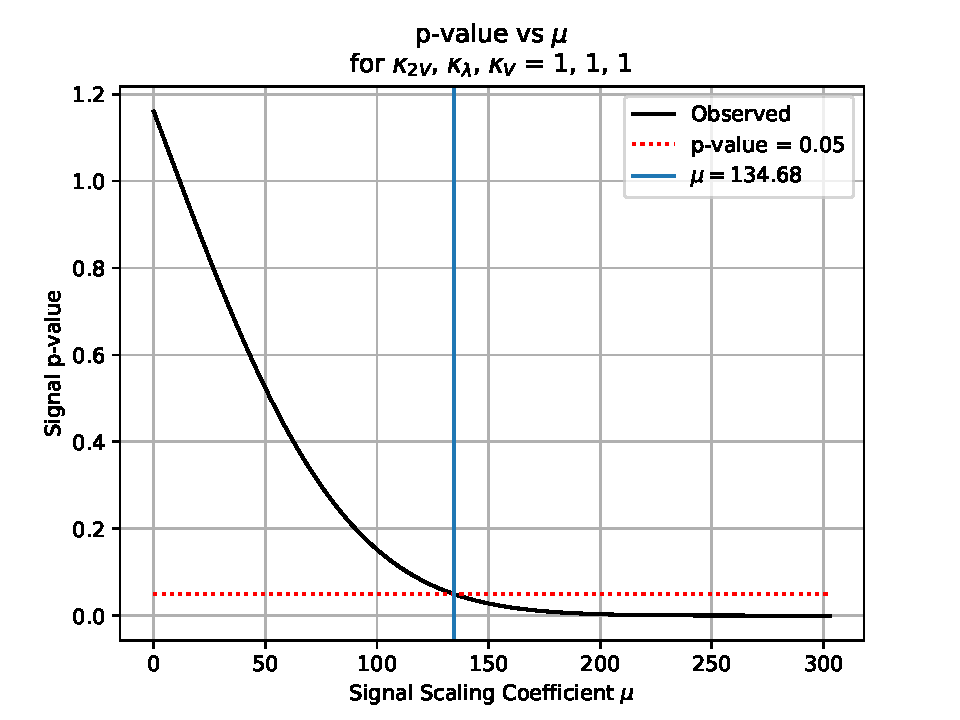
\includegraphics[width=\linewidth,height=\textheight,keepaspectratio]{results/mu_pvalue_1p00_1p00_1p00}
            \caption{}%$\mu$ Scan Plot for \kvv = 1}
            \label{fig:muscan_kvv1}
        \end{subfigure}
        \begin{subfigure}{0.48\textwidth}
            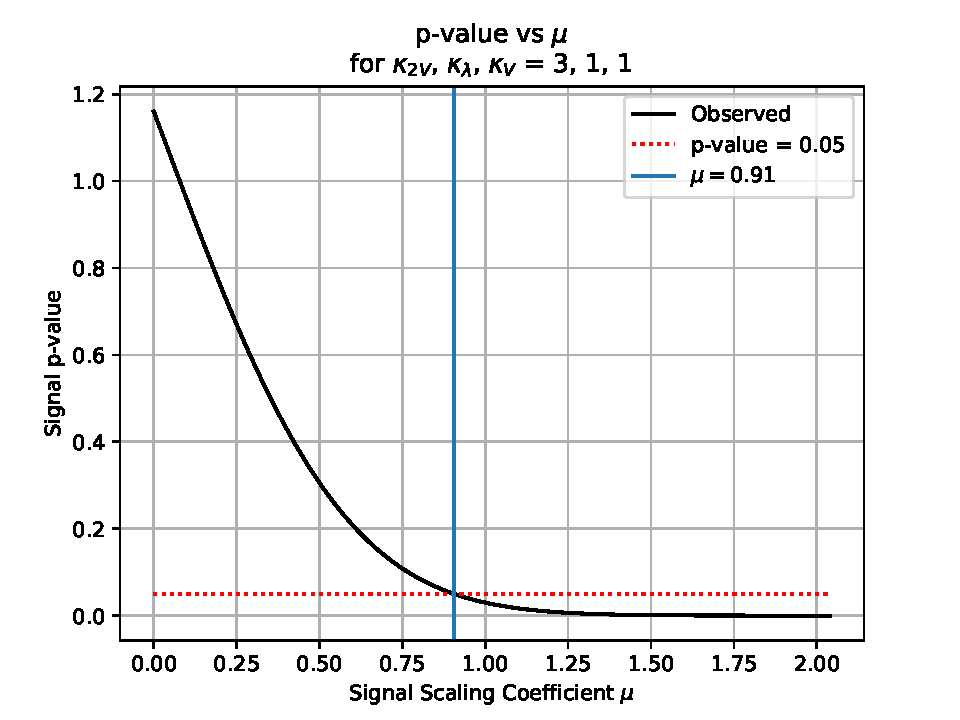
\includegraphics[width=\linewidth,height=\textheight,keepaspectratio]{results/mu_pvalue_3p00_1p00_1p00}
            \caption{}%$\mu$ Scan Plot for \kvv = 3}
            \label{fig:muscan_kvv3}
        \end{subfigure}
        \caption{
            Figures showing how the p-value of the signal hypothesis changes
                as the scaling factor $\mu$ is adjusted.
        }
    \end{figure}


    It is easy to see how this technique could be extended to arbitrary values of the $\kappa$ factors
        in order to find the precise point at which the hypothesis can be excluded.
    Utilizing the signal model linear combination equation from Section \ref{sec:signal_combination},
        the signal hypothesis for any value of \kvv can be tested, producing Fig. \ref{fig:mulimits_kvv}.
    A similar plot can be produced by scanning across the values of \kl (Fig. \ref{fig:mulimits_kl}).
    An alternate visualization of these scan plots can be produced by multiplying $\mu$ by
        the theoretical cross-section predicted for a given set of $\kappa$ factors.
    Shown in Figs. \ref{fig:xseclimits_kvv} and \ref{fig:xseclimits_kl}, these scans indicate how far the \vbfproc cross-section would have to deviated from
        the theoretical value in order to remain compatible with the observed data.

    \begin{figure}
        \centering
        \begin{subfigure}{0.48\textwidth} 
            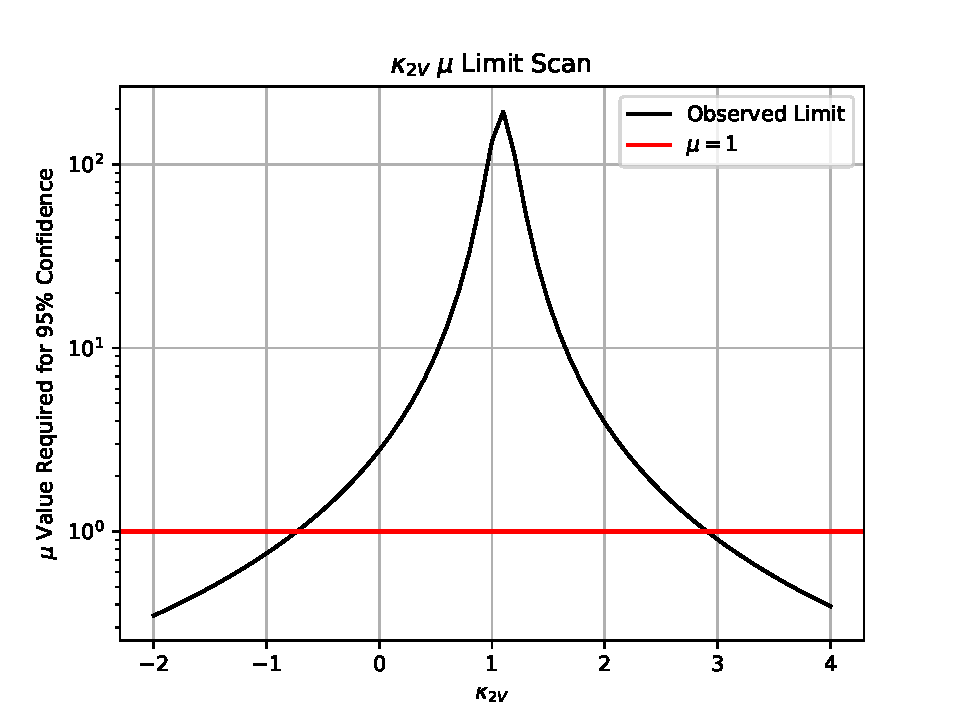
\includegraphics[width=\linewidth,height=\textheight,keepaspectratio]{results/mu_limits_fast_k2v}
            \caption{}%$\mu$ Scan Plot for \kvv = 1}
            \label{fig:mulimits_kvv}
        \end{subfigure}
        \begin{subfigure}{0.48\textwidth}
            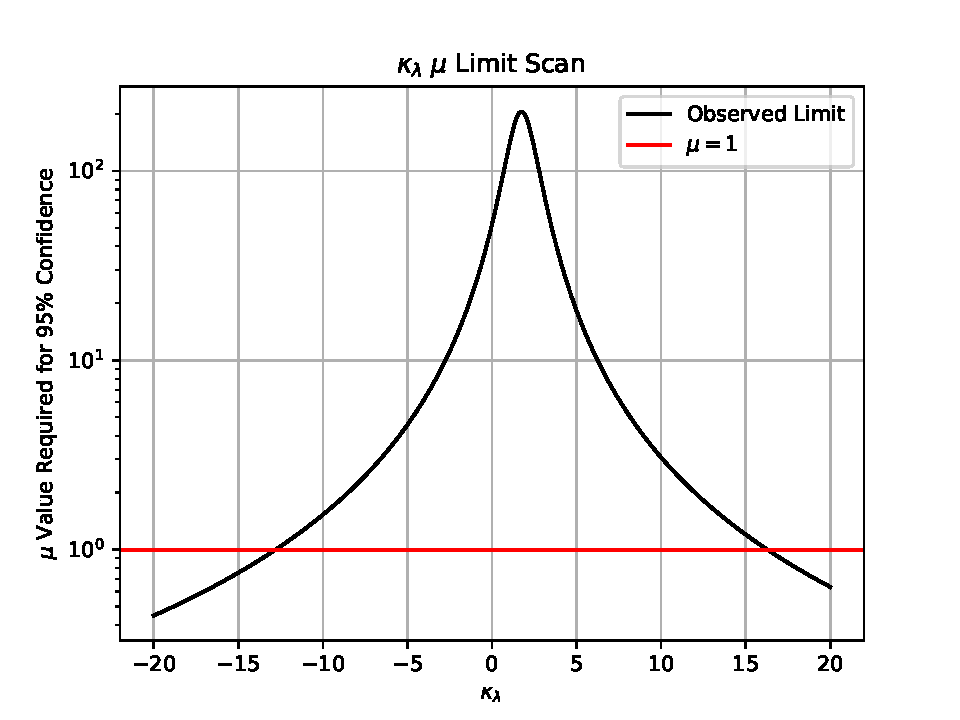
\includegraphics[width=\linewidth,height=\textheight,keepaspectratio]{results/mu_limits_fast_kl}
            \caption{}%$\mu$ Scan Plot for \kvv = 3}
            \label{fig:mulimits_kl}
        \end{subfigure}\\
        \begin{subfigure}{0.48\textwidth} 
            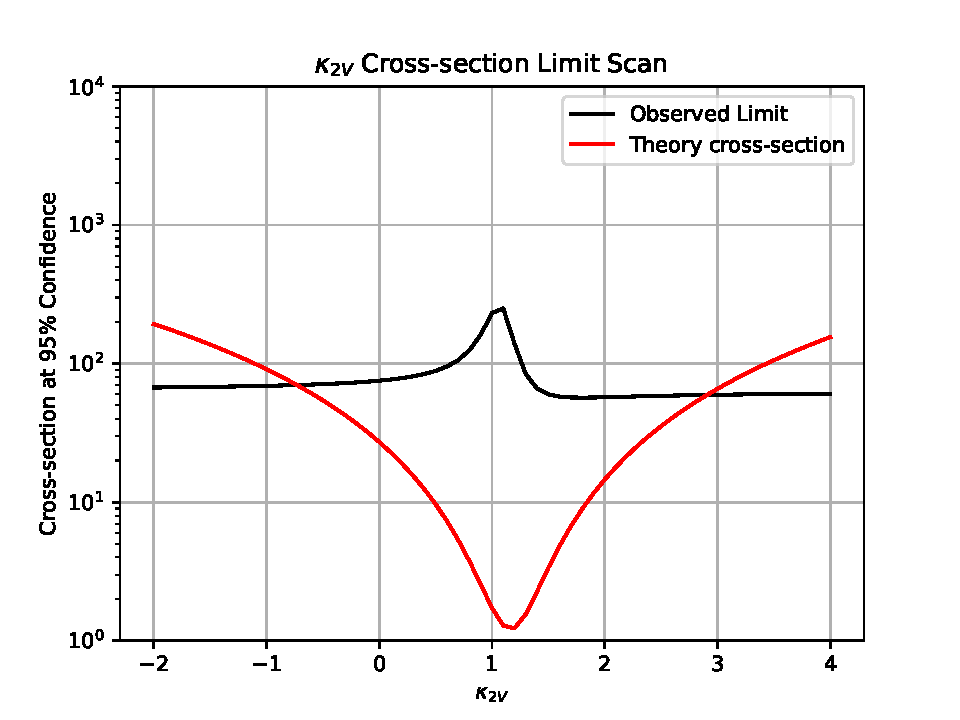
\includegraphics[width=\linewidth,height=\textheight,keepaspectratio]{results/xsec_limits_fast_k2v}
            \caption{}%$\mu$ Scan Plot for \kvv = 1}
            \label{fig:xseclimits_kvv}
        \end{subfigure}
        \begin{subfigure}{0.48\textwidth}
            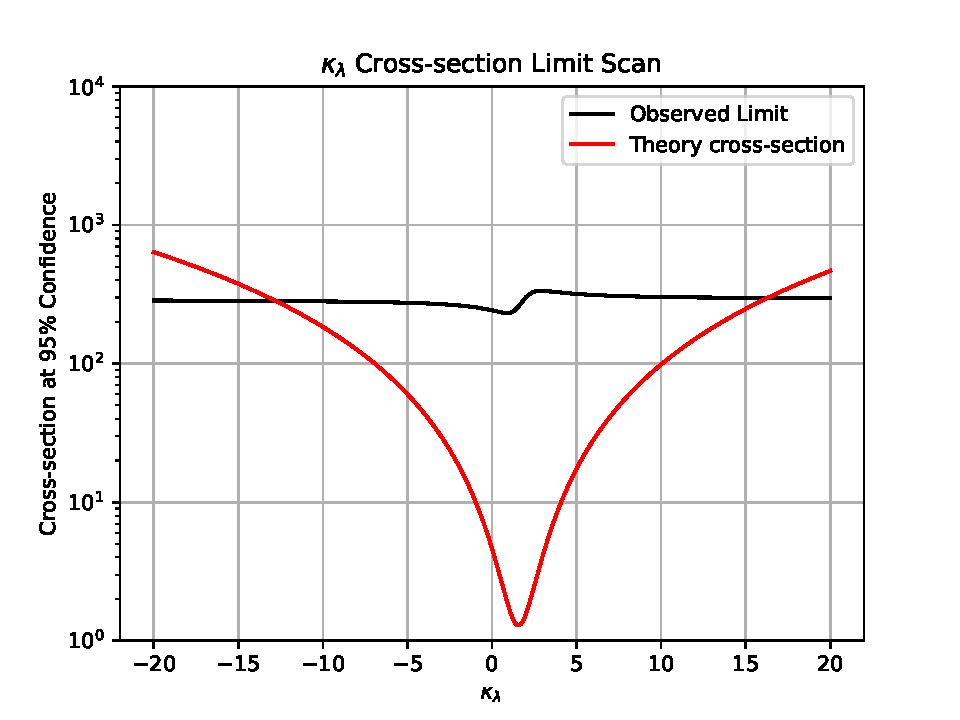
\includegraphics[width=\linewidth,height=\textheight,keepaspectratio]{results/xsec_limits_fast_kl}
            \caption{}%$\mu$ Scan Plot for \kvv = 3}
            \label{fig:xseclimits_kl}
        \end{subfigure}
        \caption{
            Figures of scans across the \kvv and \kl scaling factors,
                demonstrating how limits can be placed on the signal based on
                the signal yield exceeding what can be reasonably (with 95\% confidence)
                be accounted for in the observed data.
        }
    \end{figure}

    Of course, the linear combination equation is not constrained to variations in only one $\kappa$ factor at a time.
    Noting that the points of greatest interest are those which define the boundary between excluded and non-excluded
        values of the $\kappa$ factors, a two-dimensional plot can be produced defining the ``exclusion zone.''
    $\mu$ at this point is superfluous as the only relevant piece of information is the p-value
        associated with a particular set of the $\kappa$ factors.
    This can be taken advantage of by redefining the Poisson expectation value again,
        replacing $S$ with the full signal yield linear combination equation (Eq. \ref{eqn:vbf_hh_6term_chosen}).
    Using the shorthand form from Eq. \ref{eq:combination_general}, the Poisson expectation takes the form
    \begin{equation} \begin{split}
        \nu(\kvv,\kl,\kv) &= S(\kvv,\kl,\kv) + B \\
        \nu(\kvv,\kl,\kv) &= \vec{g}(\kvv,\kl,\kv) \bullet \vec{S} + B
        \,.
    \end{split} \end{equation}

    The two-dimensional $\kappa$ limits can be seen in Figs \ref{fig:limit_slice_kv_1p0}-\ref{fig:limit_slice_k2v_1p0},
        which span the entire three-dimensional parameter space of the $\kappa$ factors.

    \begin{figure}
        \centering
        \begin{subfigure}{0.48\textwidth} 
            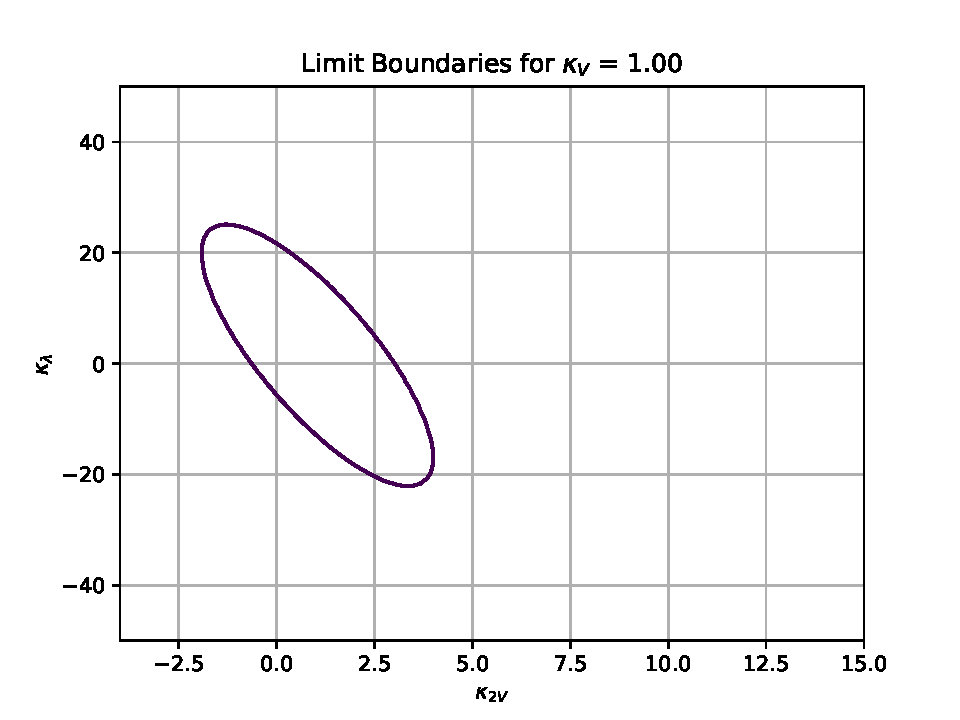
\includegraphics[width=\linewidth,height=\textheight,keepaspectratio]{results/limit_slice_kv_1p0}
            \caption{}%$\mu$ Scan Plot for \kvv = 1}
            \label{fig:limit_slice_kv_1p0}
        \end{subfigure}
        \begin{subfigure}{0.48\textwidth}
            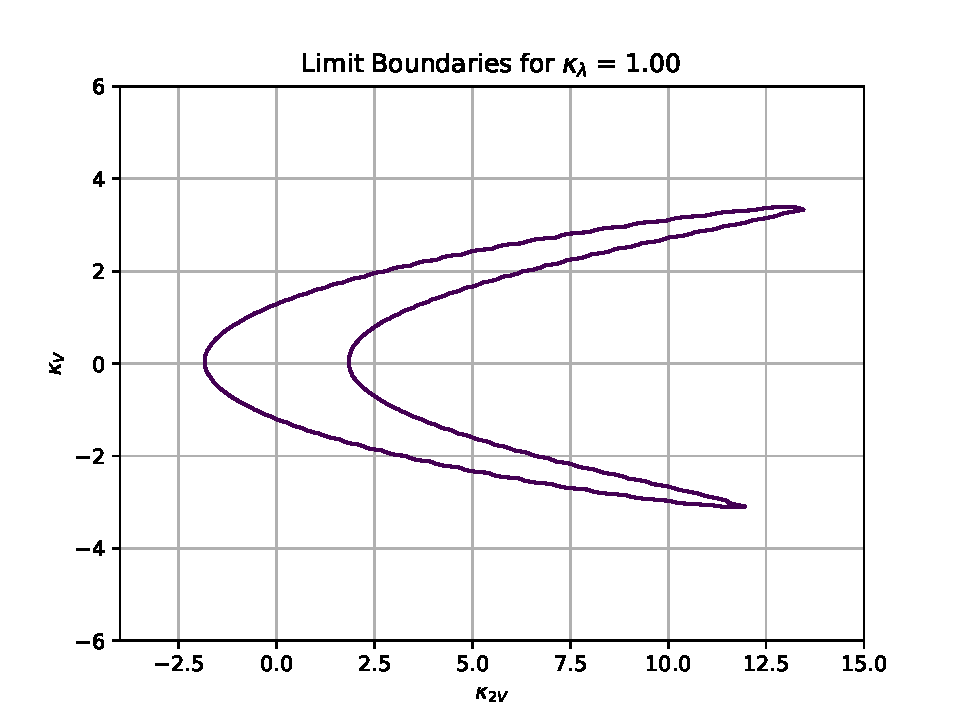
\includegraphics[width=\linewidth,height=\textheight,keepaspectratio]{results/limit_slice_kl_1}
            \caption{}%$\mu$ Scan Plot for \kvv = 3}
            \label{fig:limit_slice_kl_1p0}
        \end{subfigure}\\
        \begin{subfigure}{0.48\textwidth} 
            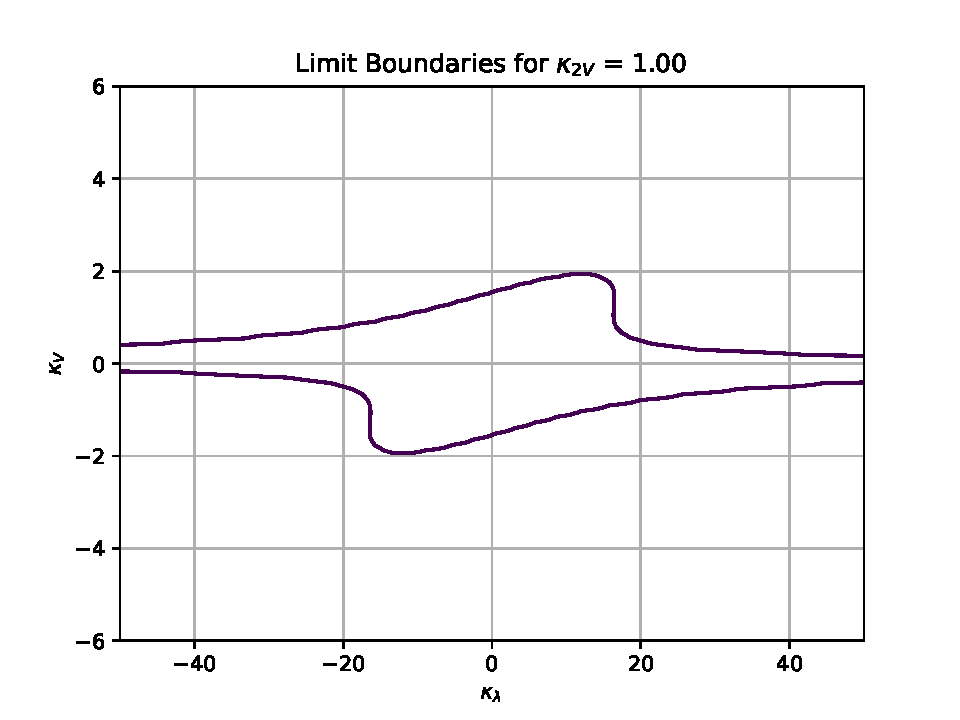
\includegraphics[width=\linewidth,height=\textheight,keepaspectratio]{results/limit_slice_k2v_1p0}
            \caption{}%$\mu$ Scan Plot for \kvv = 1}
            \label{fig:limit_slice_k2v_1p0}
        \end{subfigure}
        \caption{
            Two Dimensional Limit Exclusion plots.
            The $\kappa$ scaling factors corresponding to regions outside the limit boundary
                can be excluded based on the yield of the observed data.
            Note that the \vbfproc cross-section vanishes as \kvv and \kv both go to zero,
                hence the unconstrained ``strip'' seen along the $\kvv = \kv = 0$ axis.
        }
        \label{fig:limit_slices}
    \end{figure}

    \begin{figure}
        \centering
        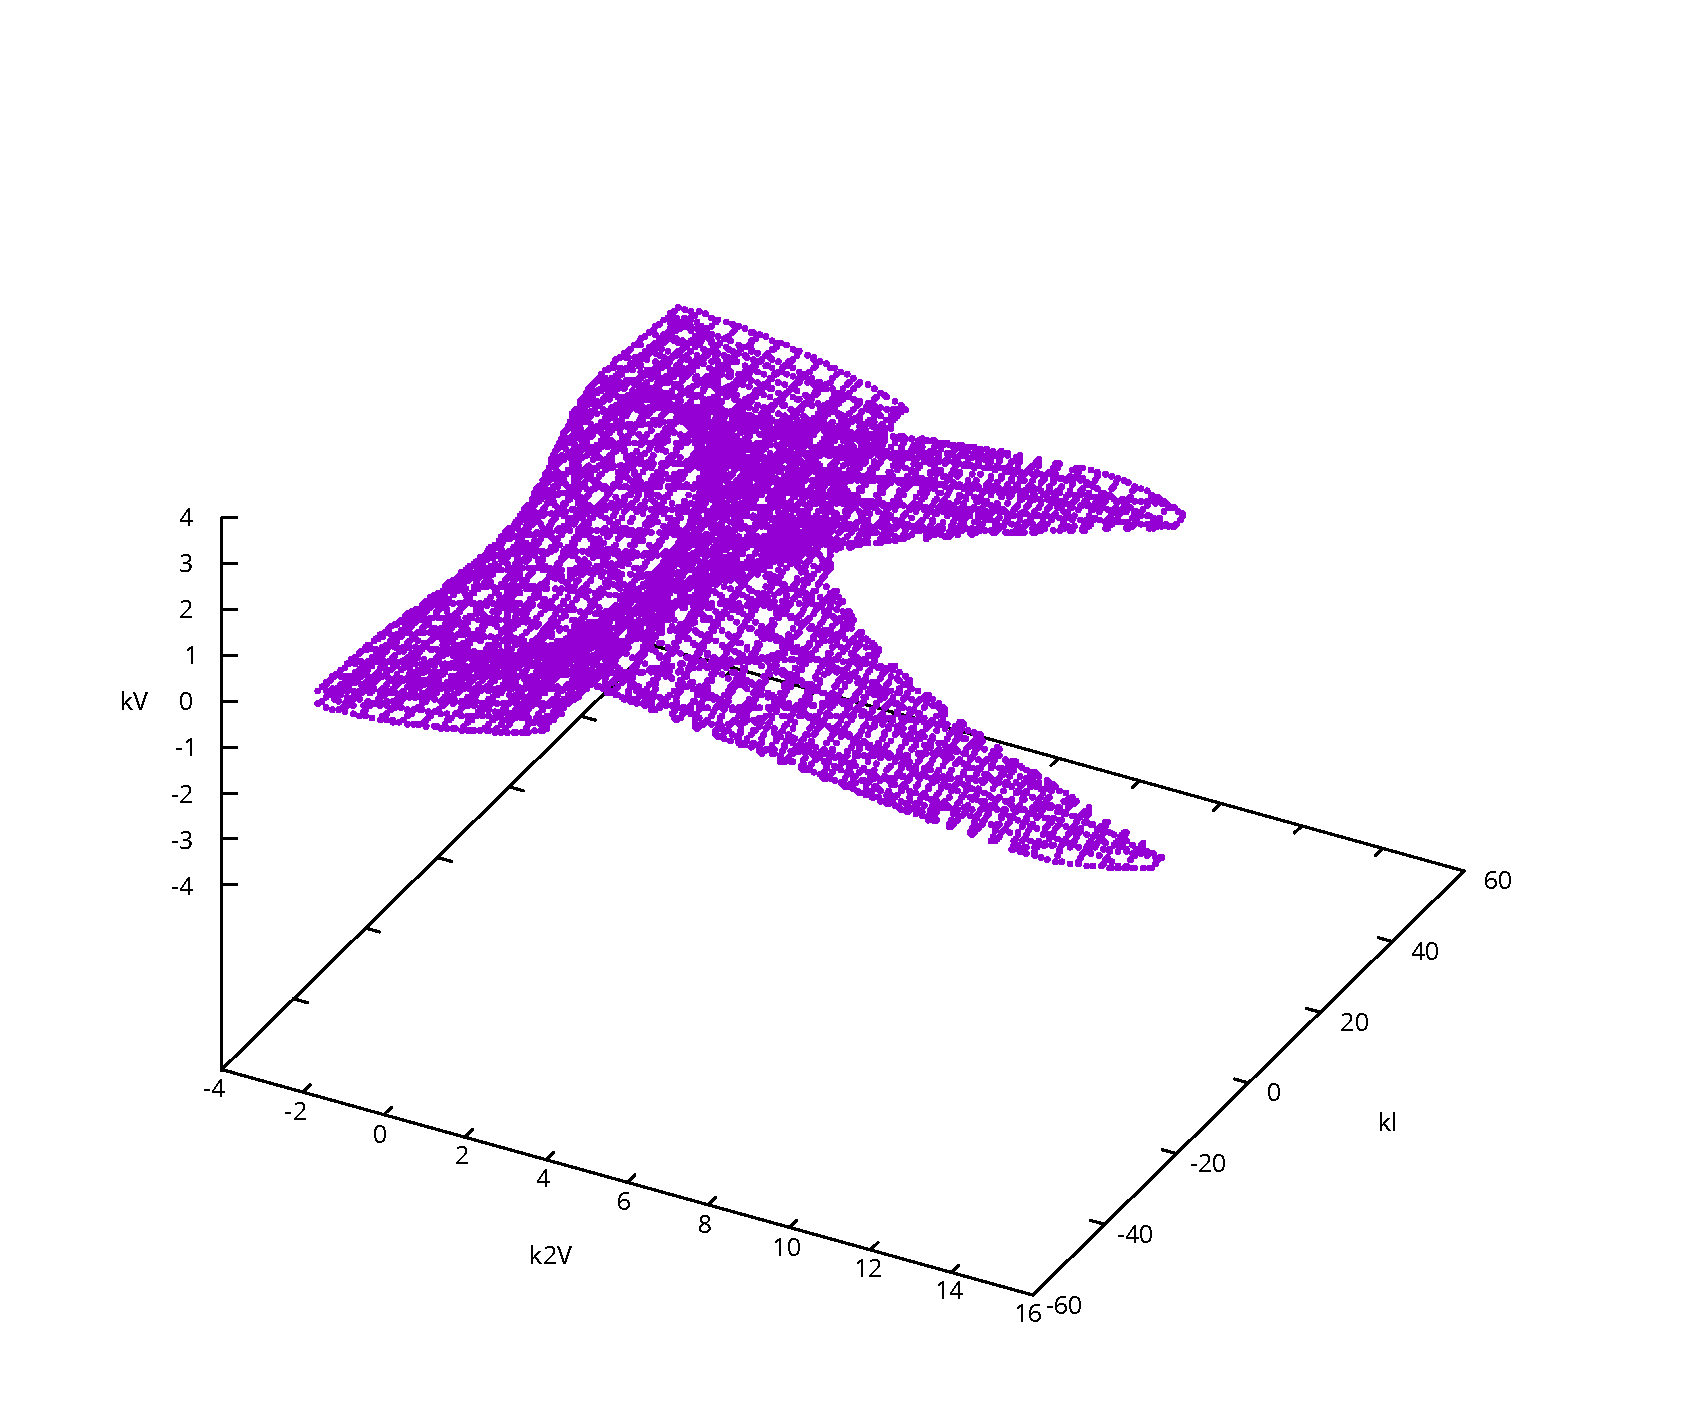
\includegraphics[width=\linewidth,height=\textheight,keepaspectratio]{results/full_3D_point_cloud}
        \label{fig:full_3D_point_cloud}
        \caption{
            A full 3D rendering of the \kvv,\kl,\kv limit exclusion region.
            The shape is highly esoteric, mostly due to the drastic effects of varying \kv far from the SM value
                (and notably well outside the bounds already set by single Higgs measurements).
            Close to the $\kv = \kvv = 0$ axis the limits extend indefinitely in \kl
                as the cross-section approaches zero,
                which renders limit-setting impossible.
        }
    \end{figure}

\FloatBarrier
% Discuss sources of error, assumptions, categorization, concept of mu values;
% basically all the complicated stuff the limit framework is doing
% Make the final goal to be establishing a p-value via the cumulative PDF distro,
%   as was done for the simple coin toss example (to bring things full circle)
\section{VBF HH 4b Limit-Setting Framework}

    Although a wealth of information can be obtained from event yields alone,
        far more statistical power can be attained by making full use of
        the kinematic information of individual events.
    The signal and background events are expected to have their events distributed differently across certain observables.
    Binning events according to their kinematic observables can emphasize these distinctions
        and highlight deviations from the null or signal hypotheses.
    In this analysis, the primary observable variable used for this purpose is the di-Higgs invariant mass, \mhh.
    Ultimately, the final test of the hypothesis will still be to create a cumulative PDF distribution,
        obtain the p-value of the cumulative PDF for the observed data, and use that to derive a CL for the signal.
    With multiple bins (as well as categories and uncertainties) however,
        the derivation of the cumulative PDF becomes much more complex.
    The following section will describe precisely how all these aspects of the analysis are combined together,
        producing a much more powerful statistical analysis.


    \begin{figure}
        \centering
        \begin{subfigure}{0.48\textwidth} 
            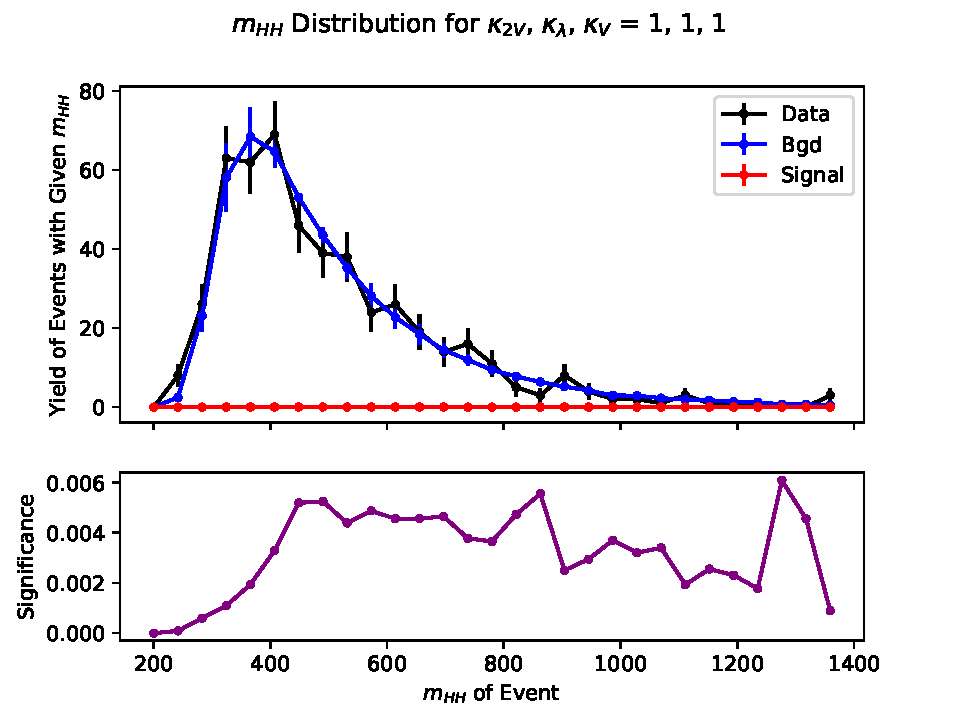
\includegraphics[width=\linewidth,height=\textheight,keepaspectratio]{results/data_dump_m_hh_1p00_1p00_1p00}
            \caption{Signal Yield Binned in \mhh for the SM}
            \label{fig:data_dump_m_hh_1p00_1p00_1p00}
        \end{subfigure}
        \begin{subfigure}{0.48\textwidth}
            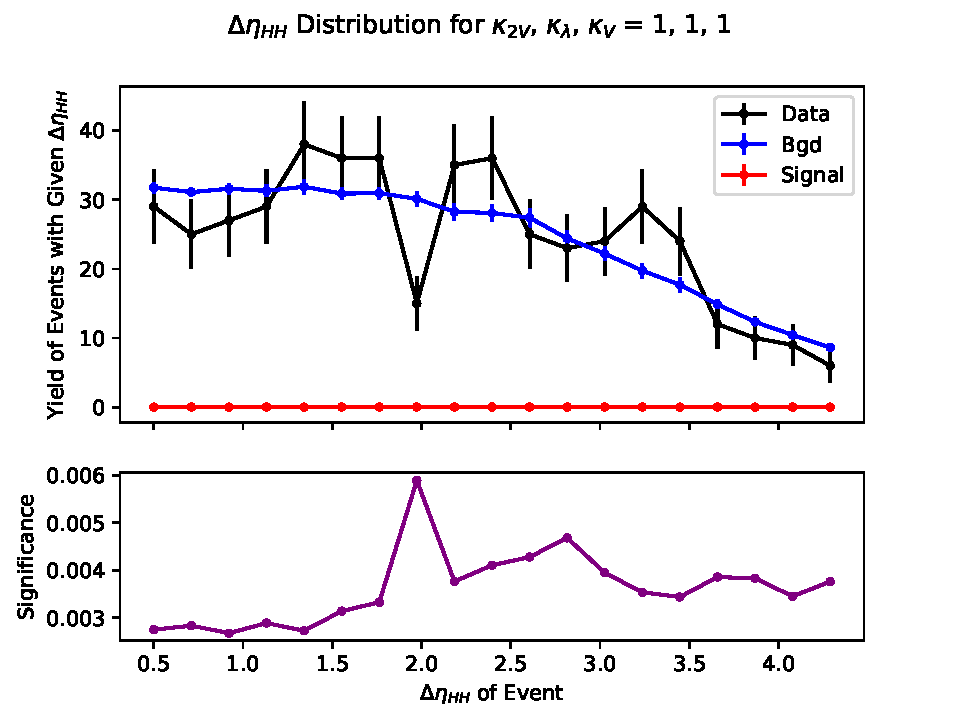
\includegraphics[width=\linewidth,height=\textheight,keepaspectratio]{results/data_dump_dEta_hh_1p00_1p00_1p00}
            \caption{Signal Yield Binned in \deta for the SM}
            \label{fig:data_dump_dEta_hh_1p00_1p00_1p00}
        \end{subfigure}\\
        \begin{subfigure}{0.48\textwidth} 
            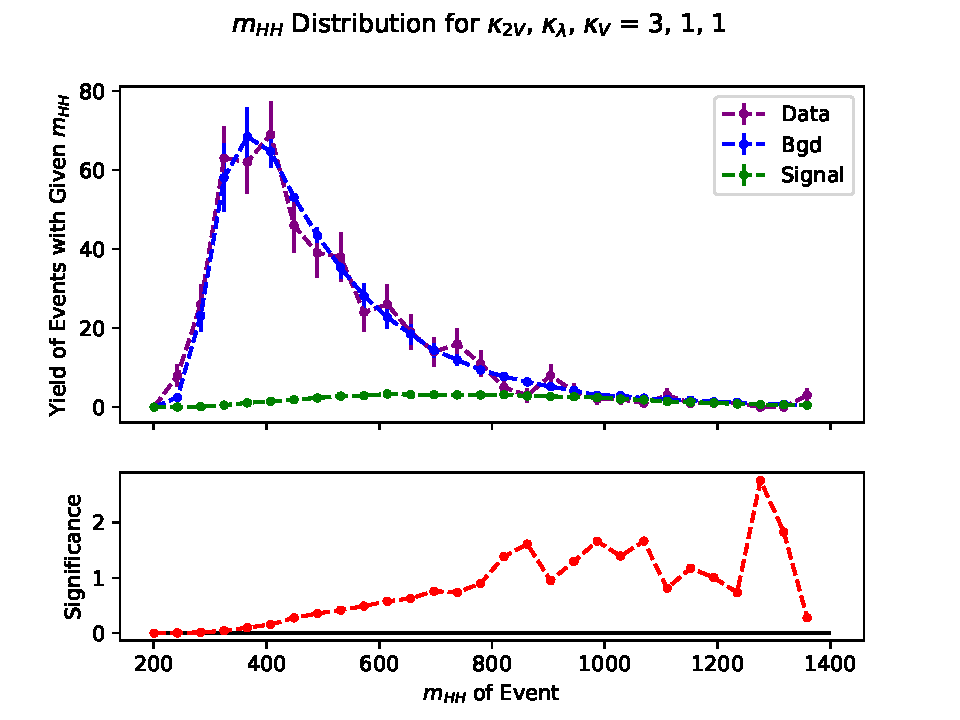
\includegraphics[width=\linewidth,height=\textheight,keepaspectratio]{results/data_dump_m_hh_3p00_1p00_1p00}
            \caption{Signal Yield Binned in \mhh for \kvv=3}
            \label{fig:data_dump_m_hh_3p00_1p00_1p00}
        \end{subfigure}
        \begin{subfigure}{0.48\textwidth}
            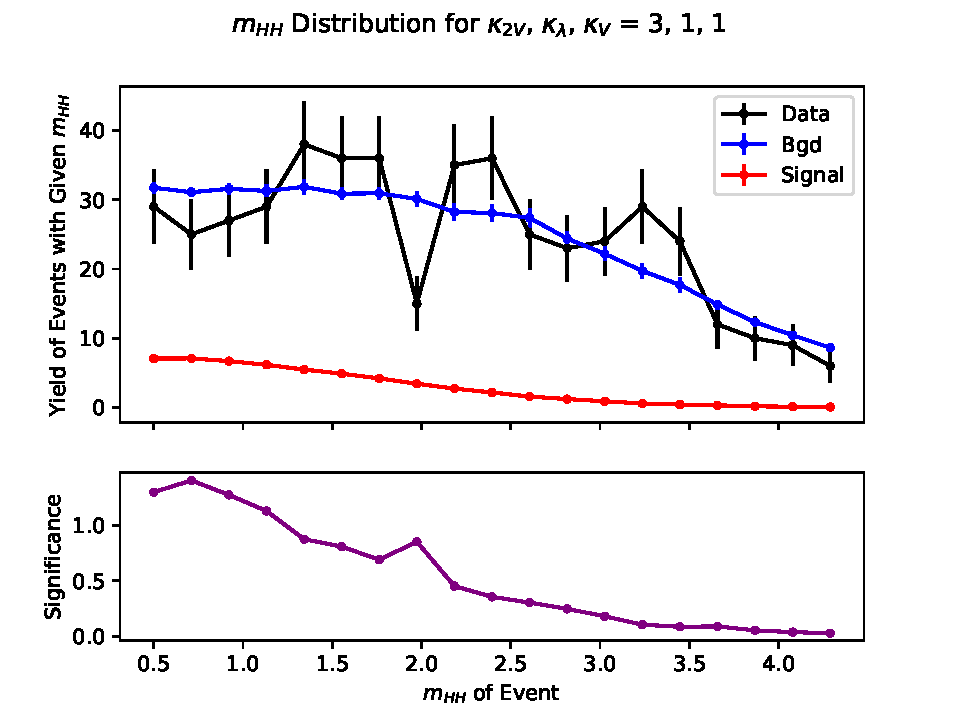
\includegraphics[width=\linewidth,height=\textheight,keepaspectratio]{results/data_dump_dEta_hh_3p00_1p00_1p00}
            \caption{Signal Yield Binned in \deta for \kvv=3}
            \label{fig:data_dump_dEta_hh_3p00_1p00_1p00}
        \end{subfigure}\\
        \begin{subfigure}{0.48\textwidth} 
            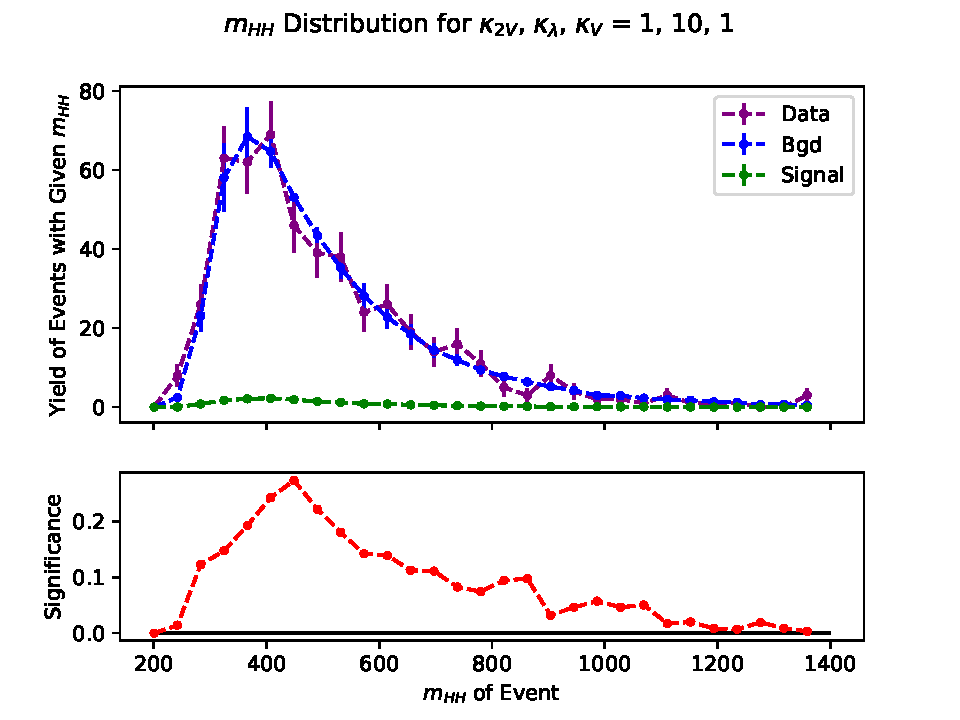
\includegraphics[width=\linewidth,height=\textheight,keepaspectratio]{results/data_dump_m_hh_1p00_10p00_1p00}
            \caption{Signal Yield Binned in \mhh for \kl=10}
            \label{fig:data_dump_m_hh_1p00_10p00_1p00}
        \end{subfigure}
        \begin{subfigure}{0.48\textwidth}
            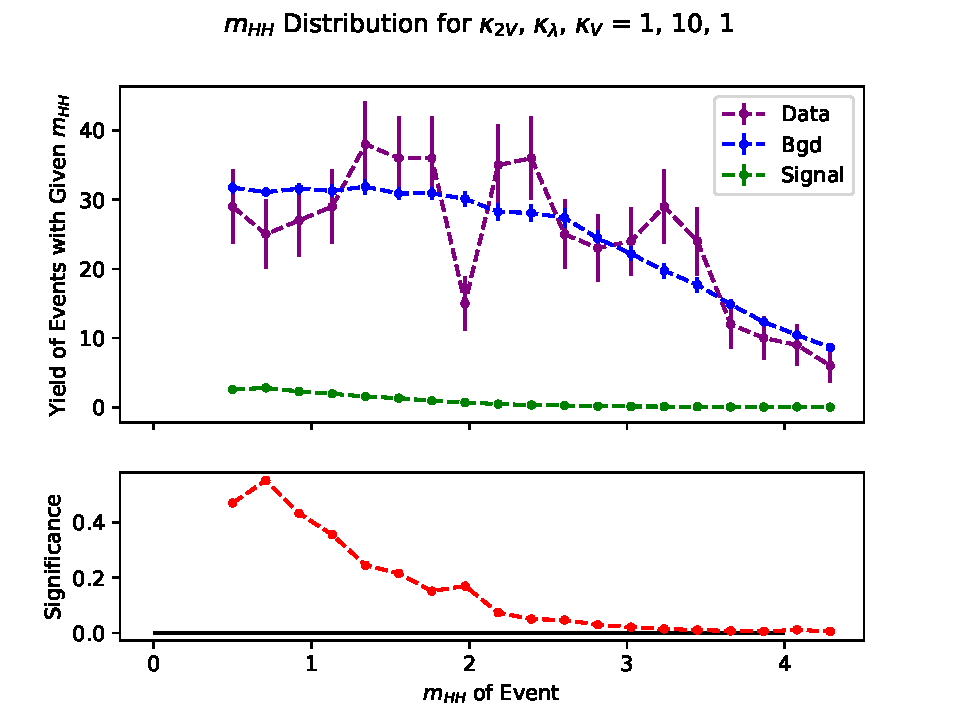
\includegraphics[width=\linewidth,height=\textheight,keepaspectratio]{results/data_dump_dEta_hh_1p00_10p00_1p00}
            \caption{Signal Yield Binned in \deta for \kl=10}
            \label{fig:data_dump_dEta_hh_1p00_10p00_1p00}
        \end{subfigure}\\
        \caption{
            \scriptsize
            The event yields of the data, background, and signal binned by their \mhh and \deta distributions.
            The bottom plot displays the ``significance'' ($Z_s=\frac{S}{\sqrt{S+B}}$)
                of the analysis in a particular bin.
            Higher significance in a region will permit that region to stand out more strongly against the background in data.
            Note the sharp increase in significance for the \kvv variation at higher values of \mhh
                (which allows \kvv to be more easily constrained than \kl),
                and the increase in significance below \deta 1.5 for both the \kvv and \kl variations
                (which is the motivation for the \deta categorization split).
        }
        \label{fig:data_dump}
    \end{figure}

    
    %What is a test statistic and why do we need it?
    The statistical technique used here to obtain a cumulative PDF
        is based on the use of a ``test statistic'' derived through a \textit{profile likelihood fit}.
    Test statistics come in many forms, but the one used here is the \qtil test statistic\cite{asymptotic_formulae_for_likelihood}.
    \qtil is technically defined in a single equation,
        but that equation involves so many parameters that it is worth breaking it down into steps.

    % Introduce mu*S+B format.
    % Discuss formula for L specifically in this analysis
    %    (emphasis on explaining the bits in parentheses):

    %    L = product[ for each category (2: eta hi and lo) 
    %        product[for each bin: poissons]
    %        * product[ nuissance params (4 for bgd shape error, 1 for norm error) ] 
    %    ]
    %    
    The first step to deriving \qtil is to slightly redefine the expectation value for the number of events 
        in terms of individual bins $i$:
    \begin{equation}
        \nu_i(\mu) = \mu S_i + B_i
        \,.
    \end{equation}
    Instead of a probability distribution function, now a ``likelihood'' function $L$ will be used,
        which is the joint probability of the observed data $n_i$ in each of the bins
        (which are in turn all Poisson-distributed data in each of the bins, with expectation value $\nu_i$)
    \begin{equation}
        L(n,\mu) = \prod \limits_{i=1}^{N} P(n_i | \nu_i)
            = \prod \limits_{i=1}^{N} \frac{ (\mu S_i + B_i)^{n_i} e^{\mu S_i + B_i} }{n_i!}
        \,.
    \end{equation}
    Where $i$ runs over all the $N$ bins.
    Note that unlike a PDF, the sum of all outcomes from the likelihood function will \textit{not} sum to unity,
        and so the likelihood function does not constitute a probability distribution function\cite{cousins2020likelihood}.

    % Discuss uncertainties and categories
    Uncertainties present in the background estimate add another layer of complexity to the likelihood function,
        because uncertain parameters must be fit as well as the parameter of interest.
    The expectation value is further adjusted to be $\nu_i(\mu, \Theta) = \mu S_i + \Theta B_i$,
        where $\Theta$ is a product of five scaling values 
    \begin{equation}
        \Theta = \prod \limits_{a=1}^{4}  \theta^a
        \,.
    \end{equation}
    These scaling values, called ``nuisance parameters,''
        correspond to the four \mhh shape uncertainties $\sigma_i^a, a\in{1,2,3,4}$
        which were described in Section \ref{sec:nn_training}.
    See Figs. \ref{fig:error_dump_sm}-\ref{fig:error_dump_kl10} for a visual comparison of the size of the statistical and systematic errors
        compared to the data and predicted signal and backgrounds.
    Here the background uncertainty is modeled as a Gaussian with expectation value $\theta^a B_i$ and standard deviation $\sigma_i^a$.
    Extending the likelihood function with the nuisance parameters produces
    \begin{equation} \begin{split}
        L(n,\mu,\Theta) &= \prod \limits_{i=1}^{N} P_{\textrm{poiss}}(n_i | \nu_i) 
             \prod \limits_{a=1}^{4} P_{\textrm{gauss}}(n_i | \nu_i, \sigma_i^a) 
        \\&= \prod \limits_{i=1}^{N} \frac{ (\mu S_i + \Theta B_i)^{n_i} e^{\mu S_i + \Theta B_i} }{n_i!} \times
            \prod \limits_{a=1}^4 \frac{1}{\sigma_i^a \sqrt{2\pi}} e^{
                -\frac{1}{2}\left(\frac{n_i- (\mu S_i + \Theta B_i)}{\sigma_i^a}\right)^2
            }
        \,.
    \end{split} \end{equation}

    Finally, in order to increase sensitivity further, events are split into two different categories
        based on whether the \deta separation between the reconstructed Higgs Bosons is greater or less than 1.5 (see Fig \ref{fig:data_dump}).
    The full likelihood function is then a product over the two categories
    \begin{equation}
        L(n,\mu,\Theta) = \prod \limits_{j=1}^{2}
             \prod \limits_{i=1}^{N} P_{\textrm{poiss}}(n_{ij} | \nu_{ij}) 
             \prod \limits_{a=1}^{4} P_{\textrm{gauss}}(n_{ij} | \nu_{ij}, \sigma_{i}^a) 
        \,.
    \end{equation}


    \begin{figure}
        \centering
        \begin{subfigure}{0.48\textwidth} 
            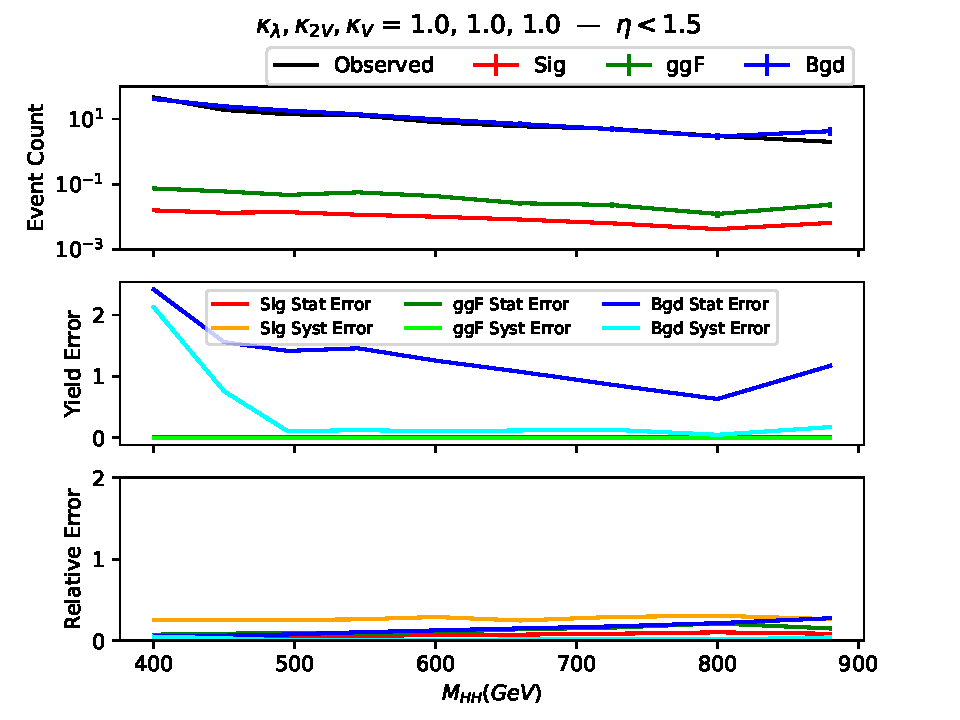
\includegraphics[width=\linewidth,height=\textheight,keepaspectratio]{results/error_comparison_kl1p0_kvv1p0_kv1p0cat0}
            \caption{Yields Binned in \mhh for the SM, $\eta < 1.5$}
            \label{fig:error_dump_eta0_1p00_1p00_1p00}
        \end{subfigure}
        \begin{subfigure}{0.48\textwidth}
            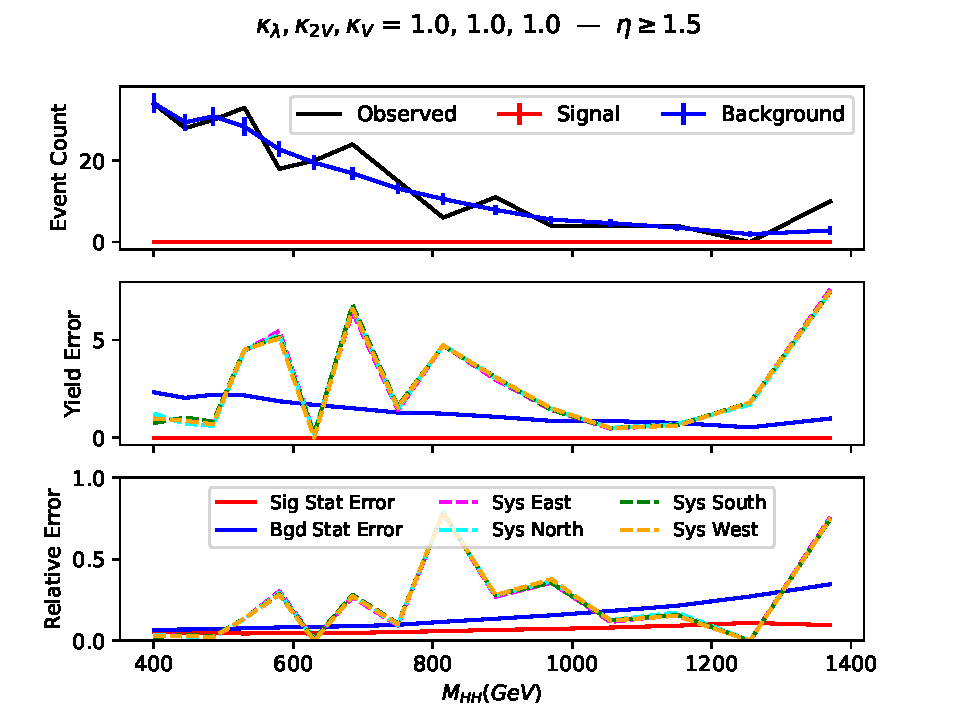
\includegraphics[width=\linewidth,height=\textheight,keepaspectratio]{results/error_comparison_kl1p0_kvv1p0_kv1p0cat1}
            \caption{Yield Binned in \deta for the SM, $\eta \geq 1.5$}
            \label{fig:error_dump_eta1_hh_1p00_1p00_1p00}
        \end{subfigure}
        \caption{
            \scriptsize
            Plots illustrating the relative scale of the data and signal/background predictions
                to the statistical and systematic errors present in this analysis,
                for both $\eta$ categories for the SM values of the $\kappa$ factors.
            The Event Count (top) plot displays event yields of data and the signal/background predictions
                with the statistical error (\textit{not} systematic) of those predictions displayed as error bars.
            Recall that the statistical error of the background is a quadrature sum of the typical stat uncertainty
                and the ``bootstrap'' uncertainty associated with the neural network training procedure.
            Also note that the statistical error of the signal is practically invisible at this scale.
            The Yield Error (middle) plot shows the values of the various errors, in units of event yields.
            The signal error continues to be basically irrelevant in comparison to the much larger
                systematic and statistical error on the background estimate.
            All four of the systematic shape uncertainties are highly consistent in their shape
                and roughly comparable to the stat uncertainty in scale.
            The jagged nature of the systematics stems from the fact that this is a background-driven estimate
                and thus statistically limited by the yield in data.
            At the bottom of the figures is the Relative Error, which shows the ratio of each of the errors
                \textit{to their respective prediction}
                (i.e.\ the signal stat error is displayed as a ratio of the signal stat error to the signal yield,
                while the background stat error is displayed as a ratio of the background stat error to the \textit{background} yield).
        }
        \label{fig:error_dump_sm}
    \end{figure}

    \begin{figure}
        \centering
        \begin{subfigure}{0.48\textwidth} 
            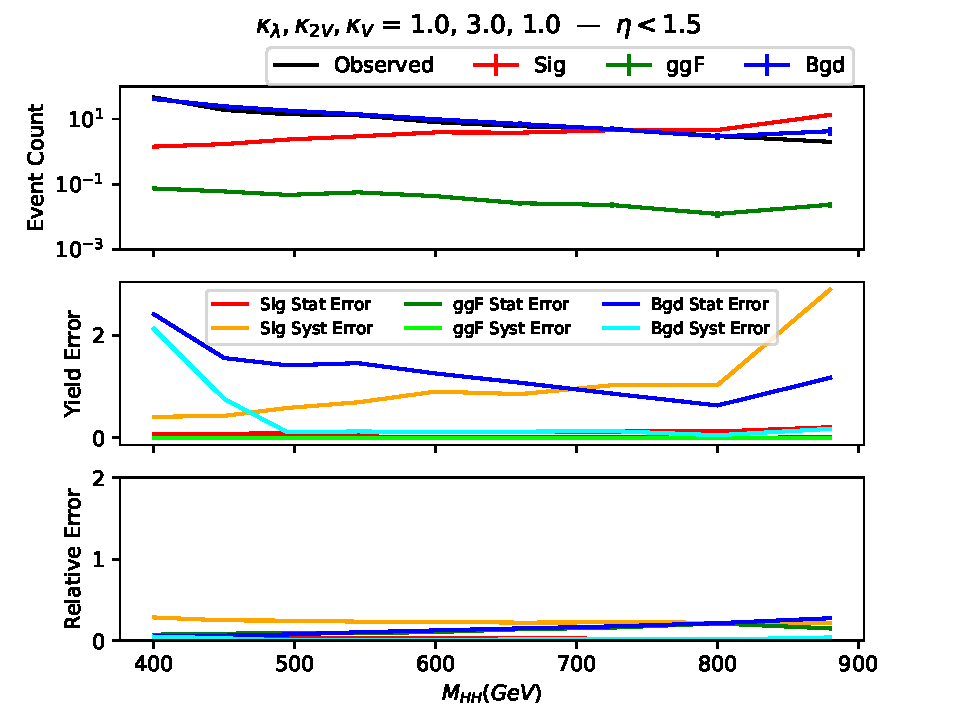
\includegraphics[width=\linewidth,height=\textheight,keepaspectratio]{results/error_comparison_kl1p0_kvv3p0_kv1p0cat0}
            \caption{Yields Binned in \mhh for \kvv=3, $\eta < 1.5$}
            \label{fig:error_dump_eta0_3p00_1p00_1p00}
        \end{subfigure}
        \begin{subfigure}{0.48\textwidth}
            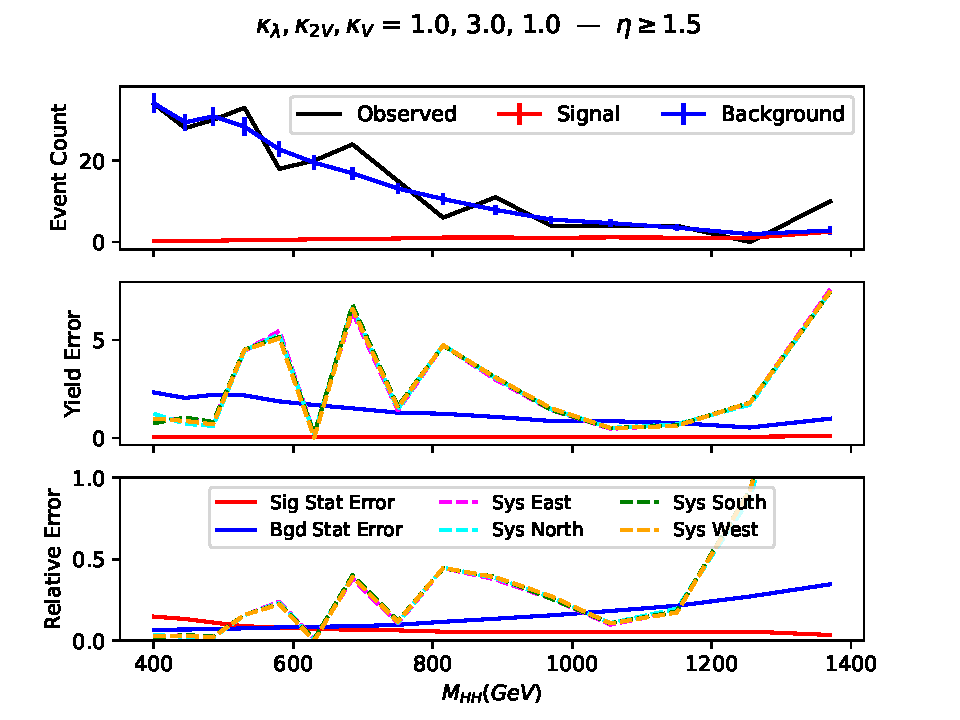
\includegraphics[width=\linewidth,height=\textheight,keepaspectratio]{results/error_comparison_kl1p0_kvv3p0_kv1p0cat1}
            \caption{Yields Binned in \deta for \kvv=3, $\eta \geq 1.5$}
            \label{fig:error_dump_eta1_hh_3p00_1p00_1p00}
        \end{subfigure}
        \caption{
            Plots illustrating the relative scale of the data and signal/background predictions
                to the statistical and systematic errors present in this analysis,
                for both $\eta$ categories for $\kvv=3$.
        }
        \label{fig:error_dump_kvv3}
    \end{figure}

    \begin{figure}
        \centering
        \begin{subfigure}{0.48\textwidth} 
            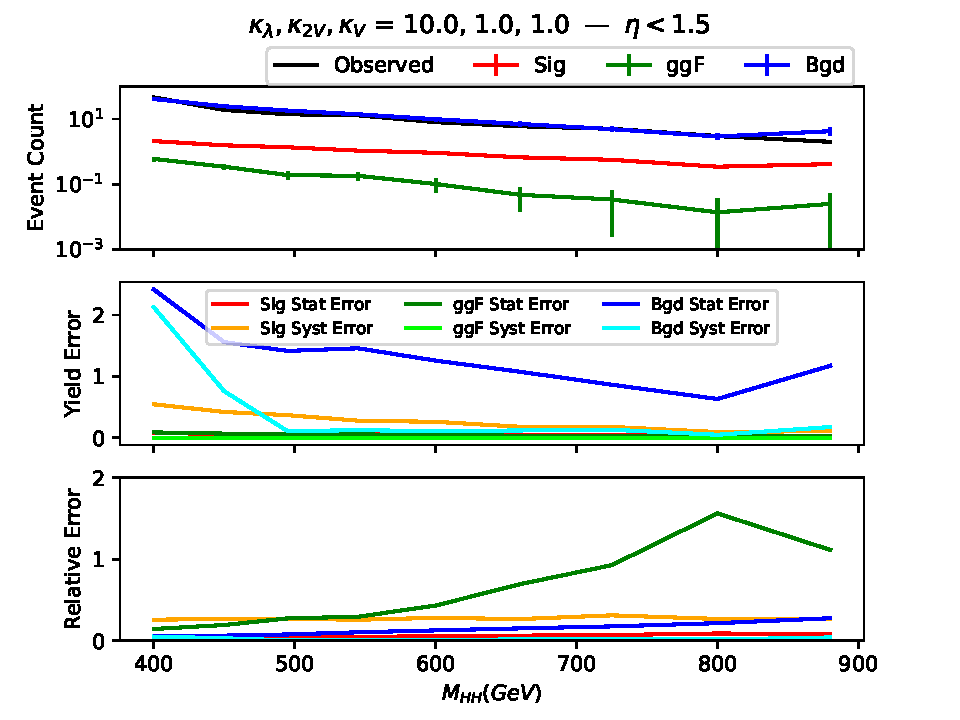
\includegraphics[width=\linewidth,height=\textheight,keepaspectratio]{results/error_comparison_kl10p0_kvv1p0_kv1p0cat0}
            \caption{Yields Binned in \mhh for \kl=10, $\eta < 1.5$}
            \label{fig:error_dump_eta0_1p00_10p00_1p00}
        \end{subfigure}
        \begin{subfigure}{0.48\textwidth}
            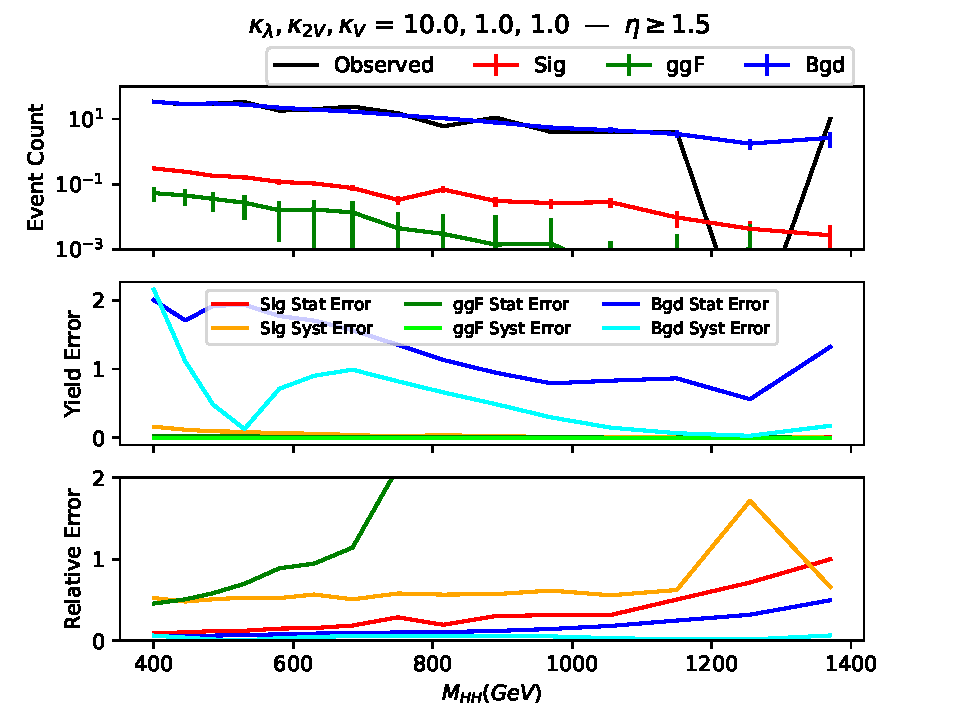
\includegraphics[width=\linewidth,height=\textheight,keepaspectratio]{results/error_comparison_kl10p0_kvv1p0_kv1p0cat1}
            \caption{Yields Binned in \deta for \kl=10, $\eta \geq 1.5$}
            \label{fig:error_dump_eta1_hh_1p00_10p00_1p00}
        \end{subfigure}
        \caption{
            Plots illustrating the relative scale of the data and signal/background predictions
                to the statistical and systematic errors present in this analysis,
                for both $\eta$ categories for $\kl=10$.
        }
        \label{fig:error_dump_kl10}
    \end{figure}


    % Discuss nuisance parameter fitting
    There is only one parameter of interest ($\mu$), but there are now six total parameters of which $L$ is a function.
    To address this without over-fitting to the data, a maximized fit is performed across the nuisance parameters.
    Such a fit eliminates their presence from the likelihood function, but it should be noted that it does so at a cost.
    The nuisance parameter fit significantly extends the final cumulative PDF, reducing the overall confidence intervals.
    To perform this fit, the value of $\mu$ is fixed to the desired scale (for now $\mu=1$),
        and then $L(n,\mu,\Theta)$ is maximized over the various values of the $\theta^a$.
    The nuisance parameter values are then fixed to this maximal value $\hat{\hat\theta}^a$, such that
    \begin{equation}
        \prod \limits_{a=1}^{4} \frac{\partial}{\partial \theta^a} L(n,\mu,\Theta) |_{\Theta=\hat{\hat\Theta}} = 0
    \end{equation}
    resulting in a fitted $L = L(n,\mu,\hat{\hat\Theta})$.
        
    %lambda = L(mu, theta vary-opt) / L(mu-opt, theta-opt);
    As a final fitting step, the likelihood $L$ is normalized to a fully maximized value $\hat L$,
        to create a quantity $\lambda = L / \hat L$.
    $\hat L$ is formed in a similar manner to $L$, but whereas $L$ has a fixed value for $\mu$,
        $\hat L$ allows $\mu$ to also be a free parameter.
    It is then maximized with regard to both $\mu$ and the nuisance parameters such that
    \begin{equation}
        \prod \limits_{a=1}^{4} \frac{\partial}{\partial \theta^a} \frac{\partial}{\partial \mu} L(n,\mu,\Theta) |_{\Theta=\hat \Theta} |_{\mu=\hat \mu} = 0
        \,.
    \end{equation}
    A test statistic $t$ can now be constructed with $\lambda$, as
    \begin{equation}
        t = -2 \ln{\lambda} = -2 \ln{\frac{L(\mu, \hat {\hat \Theta})}{L(\hat \mu, \hat \Theta)}}
        \,.
    \end{equation}
    It is worth briefly reviewing what this formula and its pieces mean before moving onto the last step.
    The likelihood $L$ is just the joint probability that every bin of the observed data would have the values they do,
        based on the modeled expectation values.
    Due to the large number of bins, $L$ will always be an extremely small number between 0 and 1.
    By construction, $\hat L$ will always be a joint probability at least as large as $L$, though still between 0 and 1.
    Their ratio $\lambda$ represents how close $L$ is to being maximally likely for the given set of observed data and models.
    $\lambda$ can at most be equal to 1, indicating that $L$ is nearly equal to $\hat L$,
        which in turn indicates that the model fits the observed data as well as it can for any given value of $\mu$.
    In turn, a value near 0 indicates that the observed data are exceedingly unlikely to have come from the model with the given $\mu$,
        compared to the much more likely model based on the optimal value of $\mu$.
    The test statistic $t$ (being the negative log of $\lambda$) then has a simple interpretation:
        values of $t$ close to 0 indicate high likelihood,
        and the higher the value of $t$ (up to infinity) the more unlikely it is that the model is compatible with the data.

    %q~ = t with edge cases;
    At last, the desired test statistic \qtil can be derived, as a piece-wise variation on $t$\cite{asymptotic_formulae_for_likelihood}:
    \begin{equation}
        \qtil = \begin{cases}
            -2 \ln{\frac{L(\mu, \hat {\hat \Theta})}{L(0, \hat \Theta(\mu=0))}} & \hat \mu < 0,\\
            -2 \ln{\frac{L(\mu, \hat {\hat \Theta})}{L(\hat \mu, \hat \Theta)}} & 0 \leq \hat \mu \leq \mu,\\
            0 & \mu < \hat \mu 
        \end{cases}
        \,.
    \end{equation}
    The middle condition is simply $t$, with the top and bottom edge cases being the defining traits of \qtil.
    \qtil in particular is used for this analysis because of these piece-wise conditions,
        which enforce the fact that $\mu$ should never be negative
        (the signal cannot remove events from the background),
        and that this analysis is only interested in establishing a lower-bound
        (and so equates as maximally likely any models for which the $\mu$ being tested is less than the optimal $\hat\mu$).

    %Single mu vs q~ PDF constructed from monte-carlo distros
    %C-PDF showing where mu-model resides for Psb, Pb, and finally Ps=Psb/(1-Pb)
    %In practice, the q~ CPDF distros are estimated using an asymptotic approximation method\cite{asymptotic_formulae_for_likelihood}.
    %(because the MC method is way too slow)
    Even with the test statistic \qtil available, its use may not be immediately obvious.
    Recall that the goal is to produce a cumulative probability distribution function,
        which can be compared against to obtain a p-value.
    In order to obtain a distribution, it must be created using Monte-Carlo techniques.
    A large number of simulated distributions can be generated,
        sampled from the modeled signal and background Poisson distributions.
    For each of these simulated ``observations'' the test statistic \qtil can be derived.
    The result is a collection of \qtil values, which together comprise a distribution.
    A cumulative probability distribution can be constructed with this distribution,
        by simply taking the fraction of simulated observations which fall below some value of the observed \qtil.
    For this analysis, the RooFit statistical framework is used to construct the test statistic and perform the
        Monte Carlo-based distribution calculation.
    Now that I finally have a robust mechanism for calculating the p-value of the di-Higgs signal hypothesis,
        the only step remaining is to use it.

    For the following plots, an ``expected limit'' is shown alongside the observed one.
    This is created by following the procedure used to obtain the observed limit,
        but replacing the observed data with the background estimate.
    In the absence of any signal (i.e.\ if the null hypothesis were true)
        this line is expected to be approximately equal to the observed limit.
    Significant deviations between the observed and expected limits thus warrant special attention,
        as they can be indicative of over or under-estimation of the background,
        or even new physics.
    The key phrase here is ``\textit{significant} deviations,'' which can be determined through
        the use of one and two standard deviation error bands associated with the expected limits.
    So long as deviations of the observed limit do not stray beyond these bands
        there is little cause for alarm.
    As can be seen in the remaining figures, there is strong agreement between what was expected
        and what has been observed, with at most only a small overestimate of the background.




    \begin{figure}
        \centering
        \begin{subfigure}{0.48\textwidth} 
            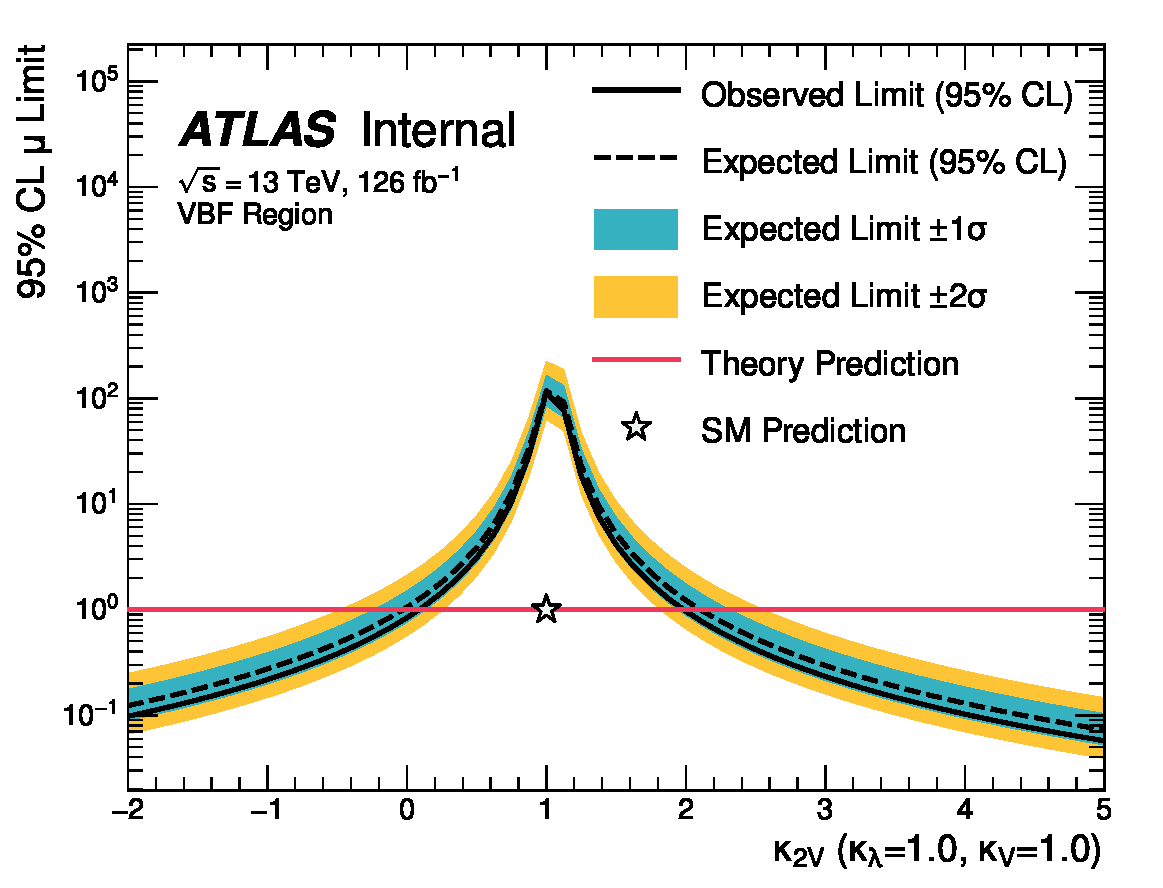
\includegraphics[width=\linewidth,height=\textheight,keepaspectratio]{results/k2v_scan_thesis_3D_samps_vbf_pd_vbf_inc161718_kl_1p0_mu}
            \caption{\kvv $\mu$ Scan}
            \label{fig:mulimits_kvv_rooFit}
        \end{subfigure}
        \begin{subfigure}{0.48\textwidth}
            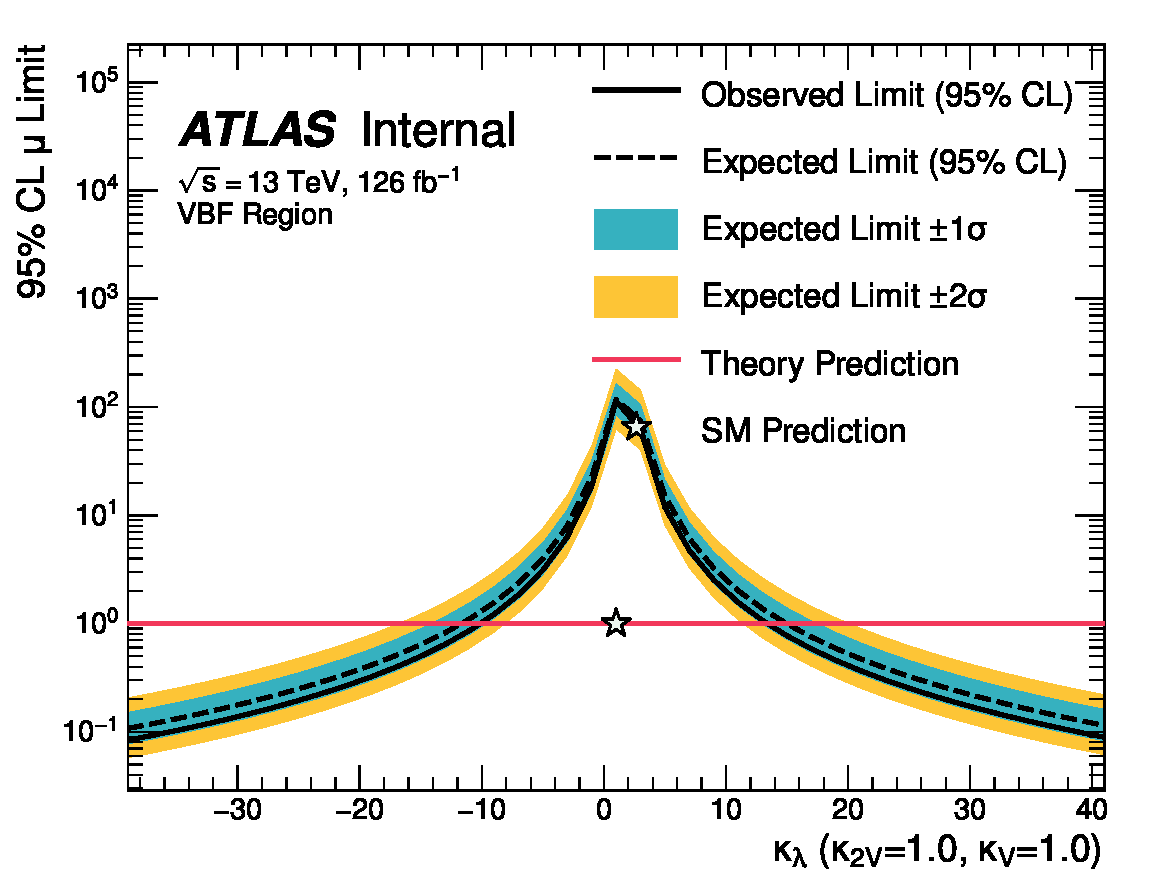
\includegraphics[width=\linewidth,height=\textheight,keepaspectratio]{results/kl_scan_thesis_3D_samps_vbf_pd_vbf_inc161718_k2v_1p0_mu}
            \caption{\kl $\mu$ Scan}
            \label{fig:mulimits_kl_rooFit}
        \end{subfigure}\\
        \begin{subfigure}{0.48\textwidth} 
            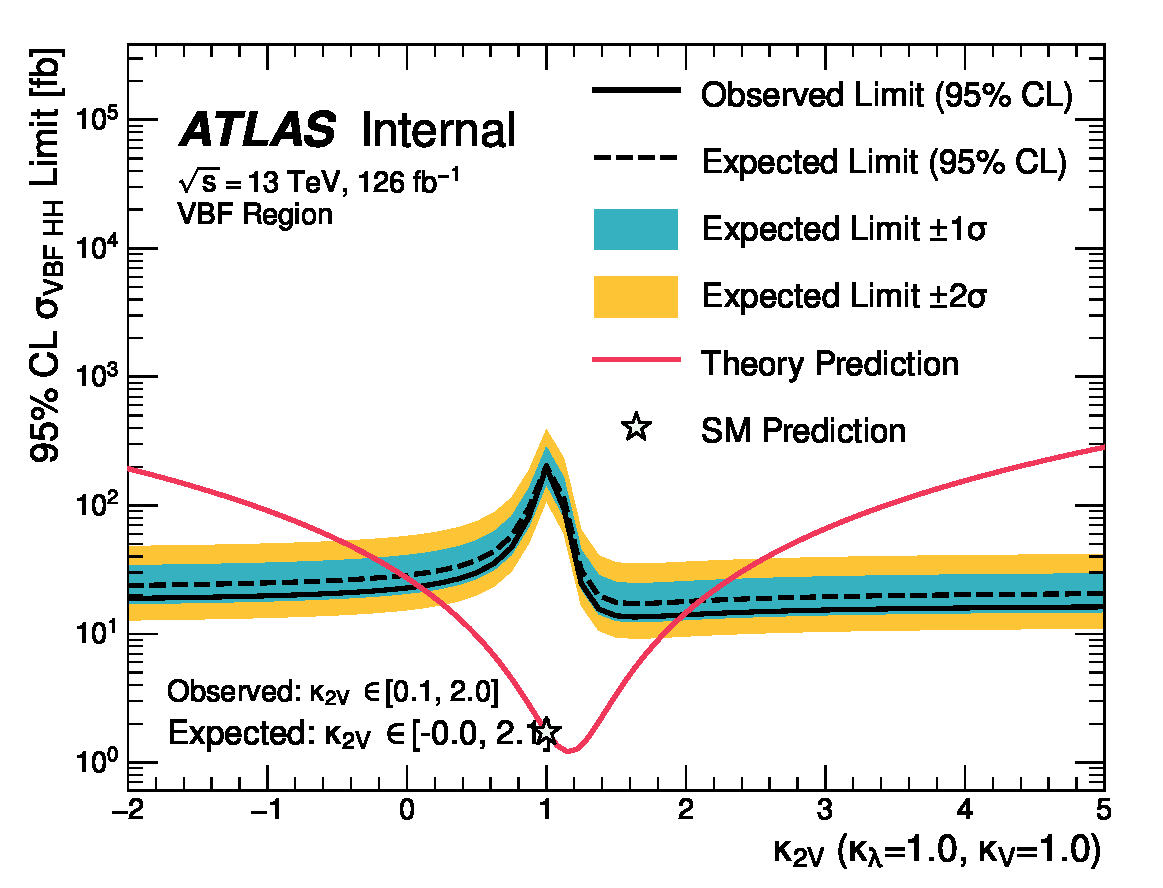
\includegraphics[width=\linewidth,height=\textheight,keepaspectratio]{results/k2v_scan_thesis_3D_samps_vbf_pd_vbf_inc161718_kl_1p0_xs}
            \caption{\kvv Cross-section Scan}
            \label{fig:xseclimits_kvv_rooFit}
        \end{subfigure}
        \begin{subfigure}{0.48\textwidth}
            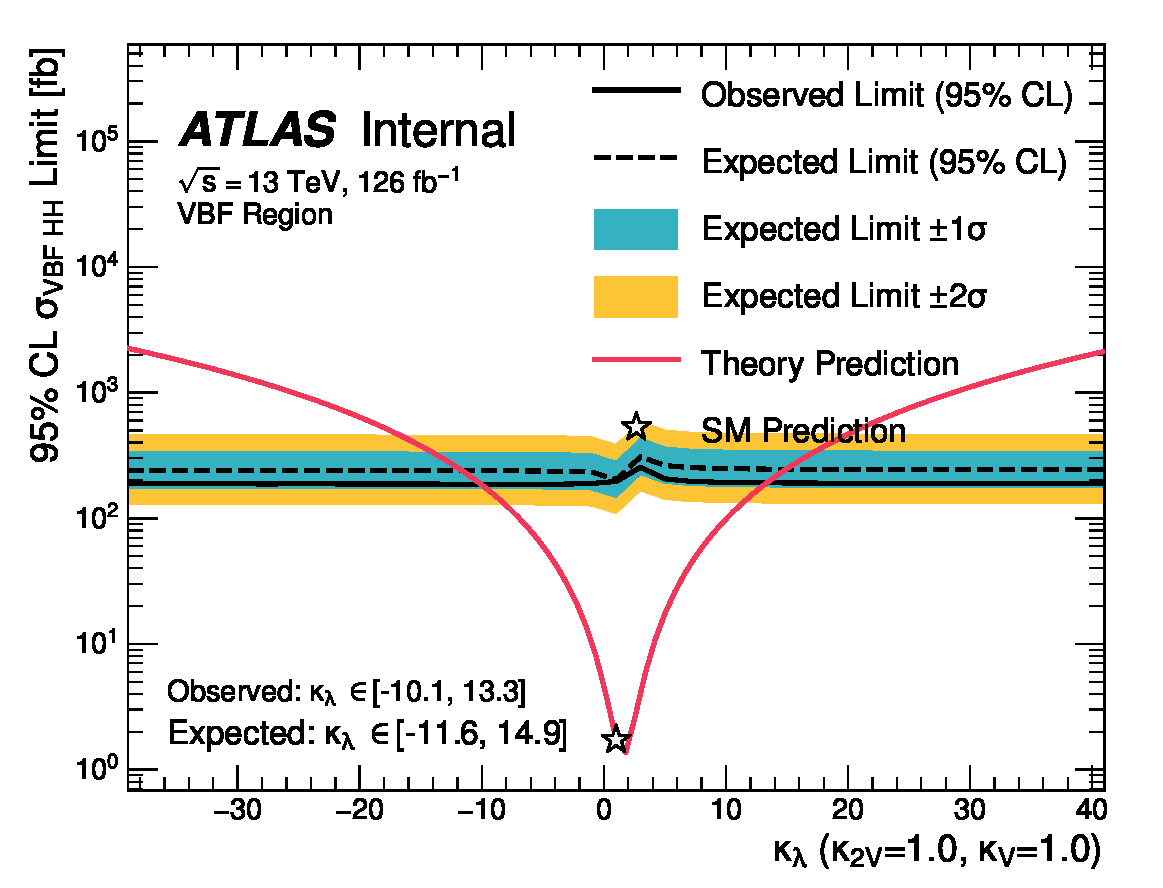
\includegraphics[width=\linewidth,height=\textheight,keepaspectratio]{results/kl_scan_thesis_3D_samps_vbf_pd_vbf_inc161718_k2v_1p0_xs}
            \caption{\kl Cross-section Scan}
            \label{fig:xseclimits_kl_rooFit}
        \end{subfigure}
        \caption{
            \kvv and \kl limit scan plots, produced using the full 4b limit setting framework.
            The limits here are much tighter than what was produced from the event yields alone.
        }
    \end{figure}


    \begin{figure}
        \centering
        \begin{subfigure}{0.48\textwidth} 
            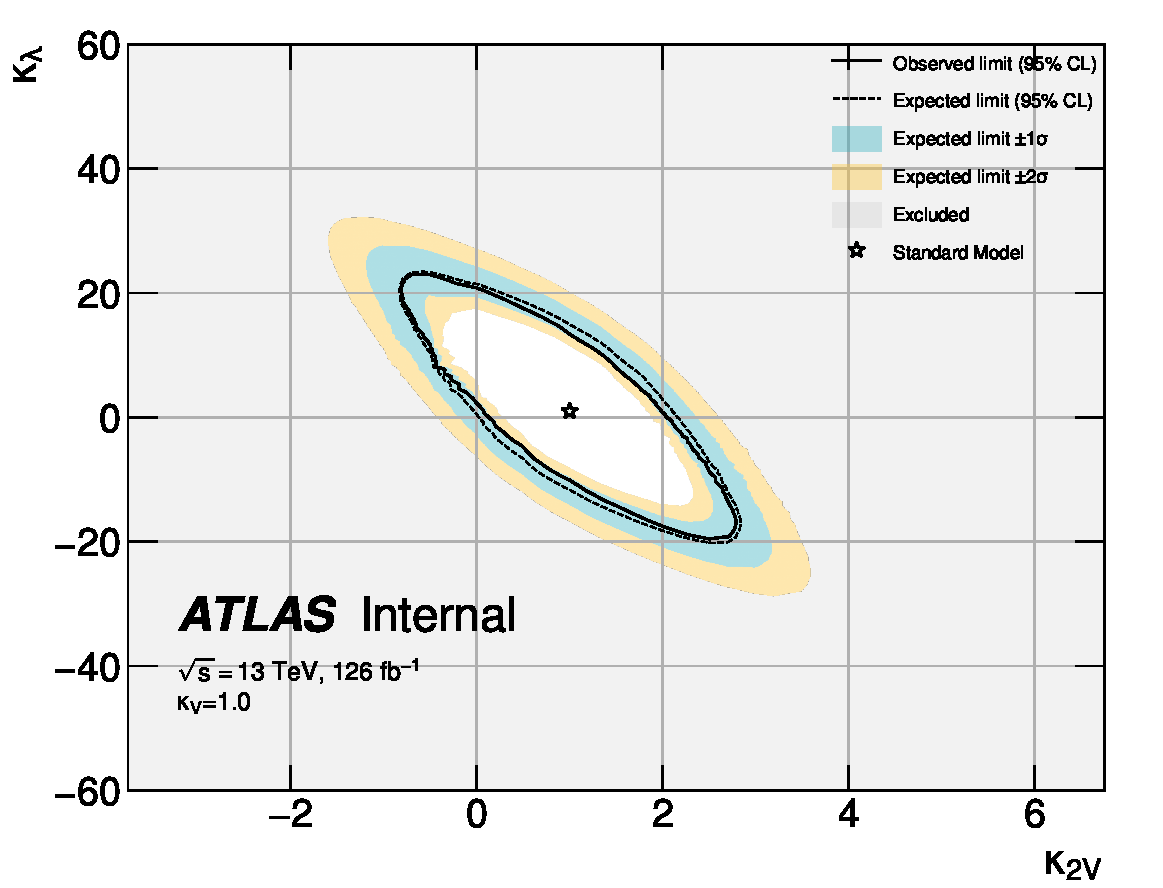
\includegraphics[width=\linewidth,height=\textheight,keepaspectratio]{results/2D_scan_thesis_omega0_kvv_kl_samps_vbf_pd_vbf_inc161718_k1v1p00_exclusion}
            \caption{2D \kvv/\kl Limit Exclusion Plot, for \kv=1}
            \label{fig:limit_slice_kv_1p0_rooFit}
        \end{subfigure}
        \begin{subfigure}{0.48\textwidth}
            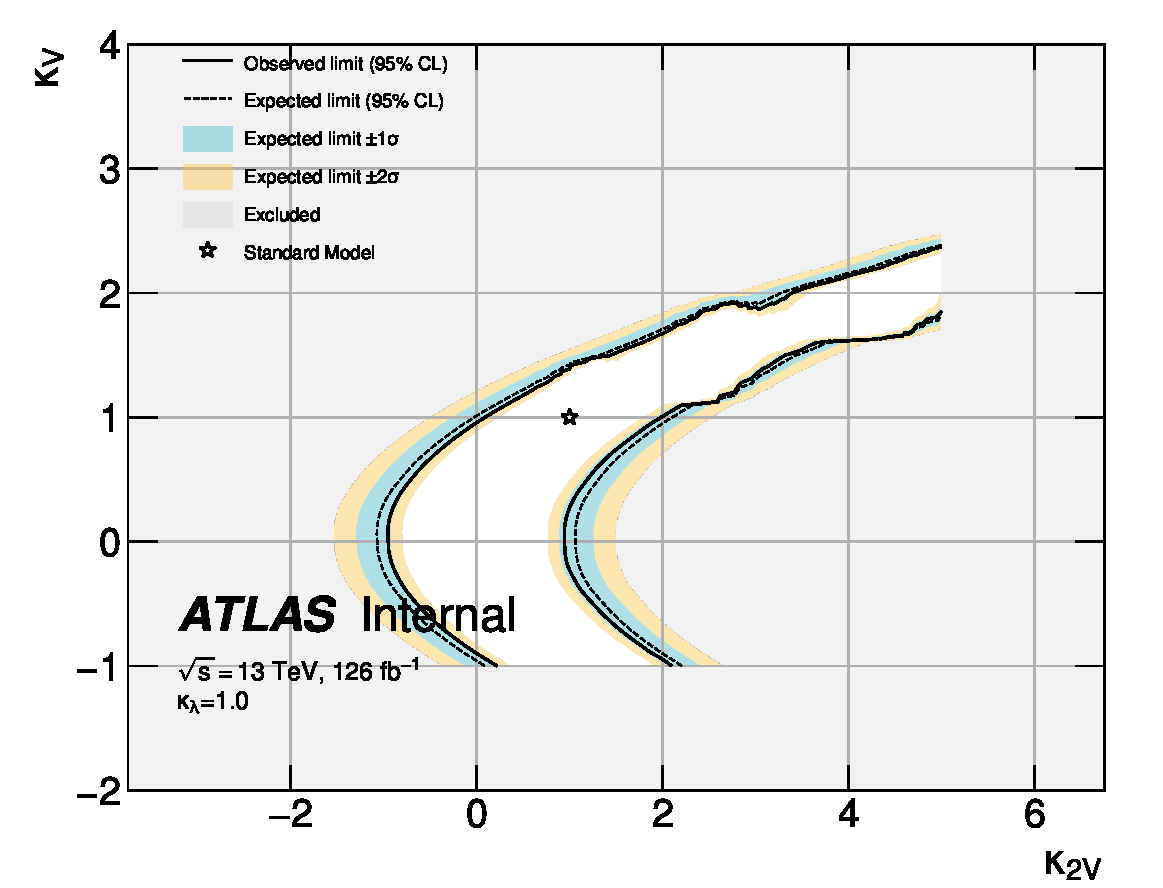
\includegraphics[width=\linewidth,height=\textheight,keepaspectratio]{results/2D_scan_thesis_omega0_kvv_kv_samps_vbf_pd_vbf_inc161718_kl1p00_exclusion}
            \caption{\kvv/\kv Limit Plot, for \kl=1}
            \label{fig:limit_slice_kl_1p0_rooFit}
        \end{subfigure}
        \caption{
            Two dimensional exclusion plots across the three $\kappa$ factors.
            The shapes are largely unchanged from those shown in Fig. \ref{fig:limit_slices},
                but are shrunken in size due to the more powerful statistical techniques used.
            The \kvv/\kv limit here is restricted between -1 and 2 due to computational constraints.
        }
    \end{figure}
